\chapter{XUV Light Source Design and Apparatus Performance}

\section{Introduction}

Compared to RABBITT measurements, condensed matter transient absorption experiments require a high XUV photon flux. First, the sample thickness is usually chosen such that the XUV transmission is roughly 50\% near the spectral feature of interest. This optical density represents a compromise between the incompatible goals of having a strong ground state absorption (enabling the detection of small changes in the optical density) while simultaneously avoiding the noise floor of the detector (which is required for good statistics). Second, a high XUV flux will reduce the number of laser shots required for a given data point, which in turn reduces the total IR flux on the sample and minimizes sample heating. Finally, a high flux reduces the overall time required to complete an experiment. This increases data fidelity by reducing the effects of unavoidable experimental noise sources such as long-term laser drift (either pointing or energy) and environmental changes caused by the building's HVAC system.

This chapter will detail the developement of bright XUV sources which were required for ATAS experiments. It will also quantify the performance of the available XUV sources and the TABLe beamline as a whole.

\section{HHG Gas Sources}
\label{sec:HHG_gas_sources}

\subsection{Scaling of Harmonic Yield}

you have a discussion of the scaling in chapter 1. consider deleting this section, or moving chap1's discussion to this location.

\subsection{Gas Flow Considerations}

- pressure in chamber requires a balance of pumping speed and gas throughput

- different gas source geometries are available: free expansion nozzle, LPC, HPC, amsterdam valve

Depending on the energy of the spectral feature, obtaining a high photon flux can range from trivial to challenging. There are many (usually interdependent) experimental parameters (gas type, interaction pressure and length, wavelength, intensity, confocal parameter, focal position relative to gas source, etc.) that can be tuned to optimize photon flux. Physically, these parameters can change the microscopic single atom response, the macroscopic coherent addition of dipole emitters (via phase matching), or both. Each experiment will usually require a unique combination of experimental settings to achieve a usable light source. For example, optimizing the harmonic yield at 100 eV for a Si L-edge measurement will usually come at the expense of harmonics yield in the 30-50 eV range, which are used to measure the transition metal M-edges.

In general, an experimentalist has neither perfect knowledge nor control over all the variables that contribute towards phase matching. Setting aside the complicated topic of phase matching, the one dimensional on-axis phase matching model\cite{constantOptimizingHighHarmonic1999} shows that the photon flux is proportional to the square of the pressure-length product of the interaction gas. That is, so long as we can remain phase matched and below the critical phase matching pressure\cite{popmintchevPhaseMatchingHigh2009}, we can universally increase the harmonic flux of our experiments by increasing the pressure-length product.

Unfortunately, one cannot ignore phase matching. Oftentimes, the spectral feature of interest lies beyond the harmonic cutoff when using the more convenient shorter wavelengths. In this case, the fundamental wavelength is increased to extend the cutoff (which scales as $\lambda^2$). However, the critical phase matching pressure also scales as $\lambda^2$ \cite{popmintchevPhaseMatchingHigh2009}, and the single atom response scales as $\lambda^{-(5-6)}$ \cite{tateScalingWavePacketDynamics2007}. These two combined effects result in a dramatically decreased photon flux if intensity and pressure are kept constant with increasing wavelength, often to the point that the resulting flux is insufficient for a transient absorption experiment, even though your cutoff has been extended to the proper energy. While some of the flux can be recovered by increasing the backing pressure of the continuous free expansion nozzle, the generation chamber's finite pumping speed limits the efficacy of pressure tuning at the longer wavelengths. Even at 800 nm, the maximum backing pressure of the continuous free expansion nozzle results in an interaction pressure below the critical phase matching pressure. Practically speaking, the continuous free expansion gas nozzle is not suitable for transient absorption experiments using the signal wavelengths ($\lambda > 1.6 \ \mu m$) or with spectral features greater than the aluminum edge at 72 eV.

Providing the lab with a brighter harmonic source was the ultimate goal of the high pressure cell, and for the most part this goal was achieved. Below, we will review the basic design considerations, drawbacks and advantages of the four main types of gas sources used in this thesis: the free expansion nozzle, the low pressure cell (LPC), the high pressure cell (HPC) and the Amsterdam pulsed piezovalve. A primer on how to install and use the high pressure cell can be found in Appendix \ref{appendix:TABLe_manual}.

\subsection{Free Expansion Nozzle}
%outline of gas jet physics:
%- why supersonic? basic physics argument
%- outline of derivation to get to the T/P/rho relationships
%- outline of derivation to get to the centerline equations
%- mach disk location, description, thickness
%- derivation of gas nozzle throughput T
%
%\begin{figure}
%	\centering
%	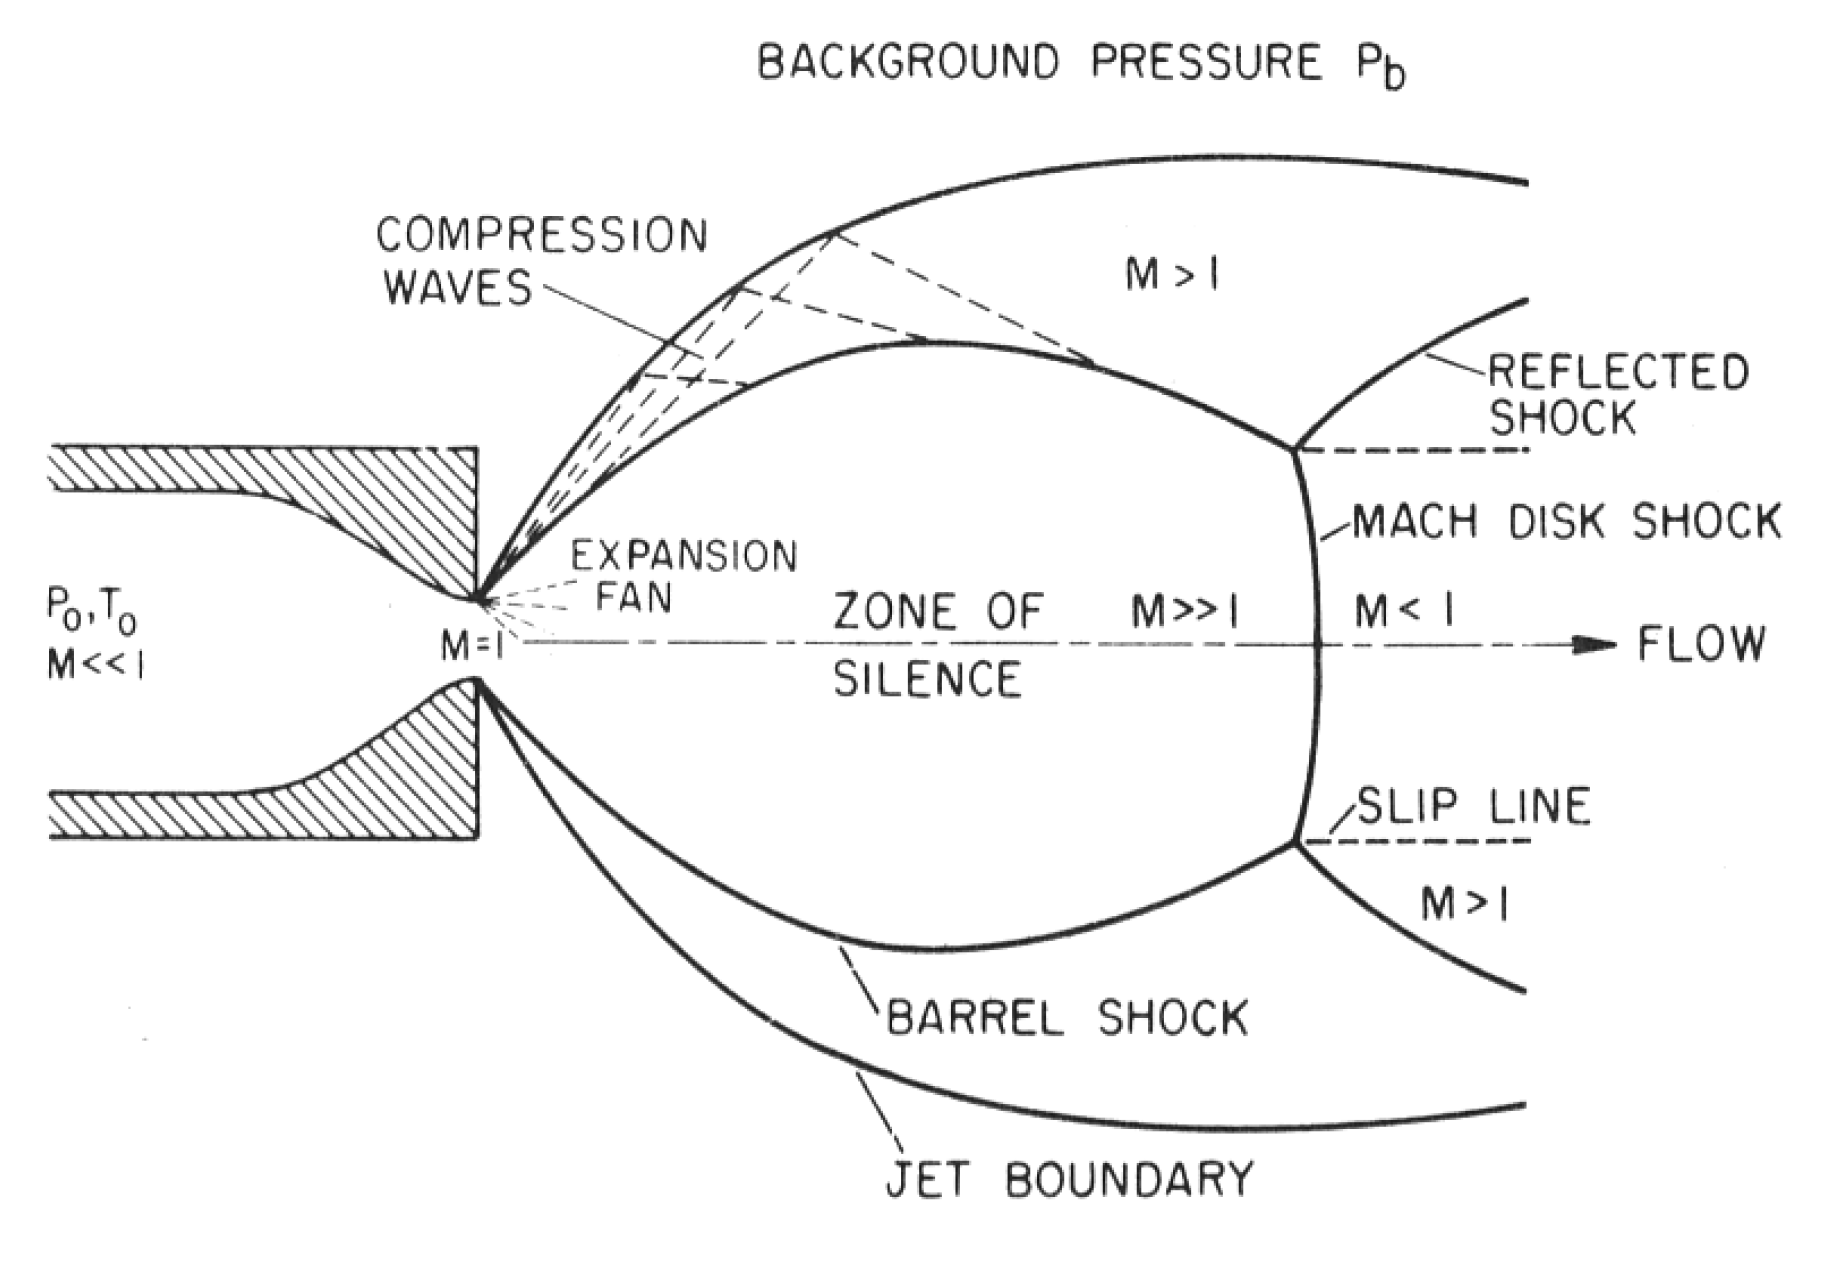
\includegraphics[width=0.5\textwidth]{figures/chap3/gas_expansion.PNG}
%	\caption{The structure of the supersonic gas plume after leaving a gas nozzle. This figure was taken from Ref \cite{millerFreeJetSources1988}.}
%	\label{fig:gas_expansion}
%\end{figure}

\begin{table}[]
	\centering
	\begin{tabular}{lllllllll}
		\hline
		\multicolumn{1}{c}{Source} & \multicolumn{1}{c}{$j$} & \multicolumn{1}{c}{$\gamma$} & \multicolumn{1}{c}{$C_1$} & \multicolumn{1}{c}{$C_2$} & \multicolumn{1}{c}{$C_3$} & \multicolumn{1}{c}{$C_4$} & \multicolumn{1}{c}{$A$} & \multicolumn{1}{c}{$B$} \\ \hline
		3D                         & 1                     & 5/3                          & 3.232                     & -0.7563                   & 0.3937                    & -0.0729                   & 3.337                & -1.541                \\
		3D                         & 1                     & 7/5                          & 3.606                     & -1.742                    & 0.9226                    & -0.2069                   & 3.190                 & -1.610                \\
		3D                         & 1                     & 9/7                          & 3.971                     & -2.327                    & 1.326                     & -0.311                    & 3.609                 & -1.950                \\
		2D                         & 2                     & 5/3                          & 3.038                     & -1.629                    & 0.9587                    & -0.2229                   & 2.339                 & -1.194                \\
		2D                         & 2                     & 7/5                          & 3.185                     & -2.195                    & 1.391                     & -0.3436                   & 2.261                 & -1.224                \\
		2D                         & 2                     & 9/7                          & 3.252                     & -2.473                    & 1.616                     & -0.4068                   & 2.219                 & -1.231               
	\end{tabular}
	\caption{Gas parameters used in \cref{eqn:Scoles_centerline2.2}. Table recreated from Ref \cite{millerFreeJetSources1988}.}
	\label{tbl:Scoles_gas_params2.2}
\end{table}

\begin{figure}
	\centering
	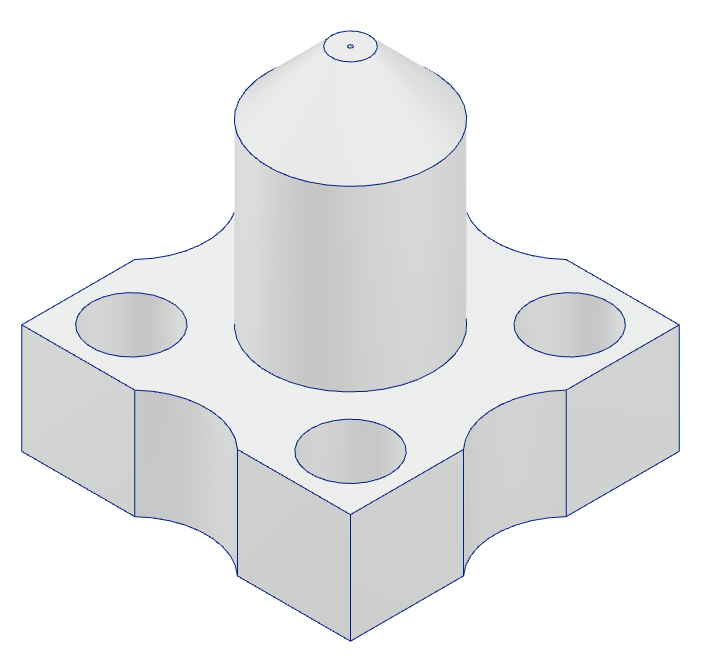
\includegraphics[width=0.5\textwidth]{figures/chap3/gas_nozzle.png}
	\caption{Rendering of the continuous free expansion nozzle. Gas flows from the base of the nozzle (bottom) and out of the 200 $\mu$m aperture (top). The top surface is beveled so the nozzle can be brought closer to the IR focus without clipping the beam.}
	\label{fig:gas_nozzle}
\end{figure}

\begin{figure}
	\centering
	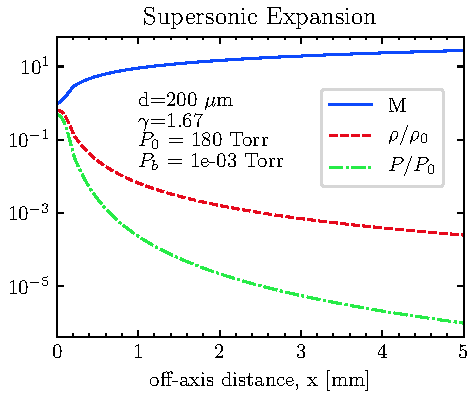
\includegraphics[width=0.75\textwidth]{figures/chap3/M_rho_P_vs_x.pdf}
	\caption{On-axis Mach number $M$, mass density $\rho$ and pressure $P$ for a free expansion nozzle.}
	\label{fig:M_rho_vs_x}
	% \Python Scripts\HPC\HPCvsLPC.py
\end{figure}

\begin{figure}
	\centering
	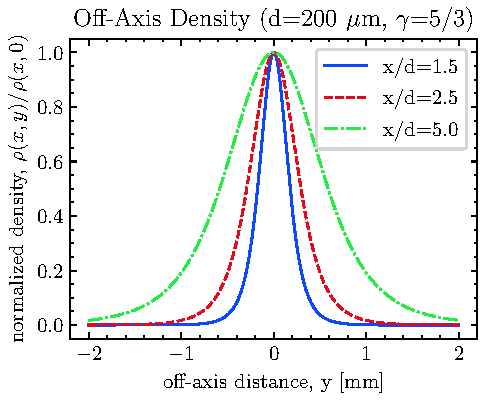
\includegraphics[width=0.75\textwidth]{figures/chap3/off_axis_density.pdf}
	\caption{Off-axis mass density $\rho(x,y)$ for various on-axis distances $x$. For an aperture size of $d = 200 \ \mu$m, the FWHM of the plume density is $120 \ \mu$m at $y = 100 \ \mu$m.}
	\label{fig:off_axis_density}
	% \Python Scripts\HPC\HPCvsLPC.py
\end{figure}

%\begin{figure}
%	\centering
%	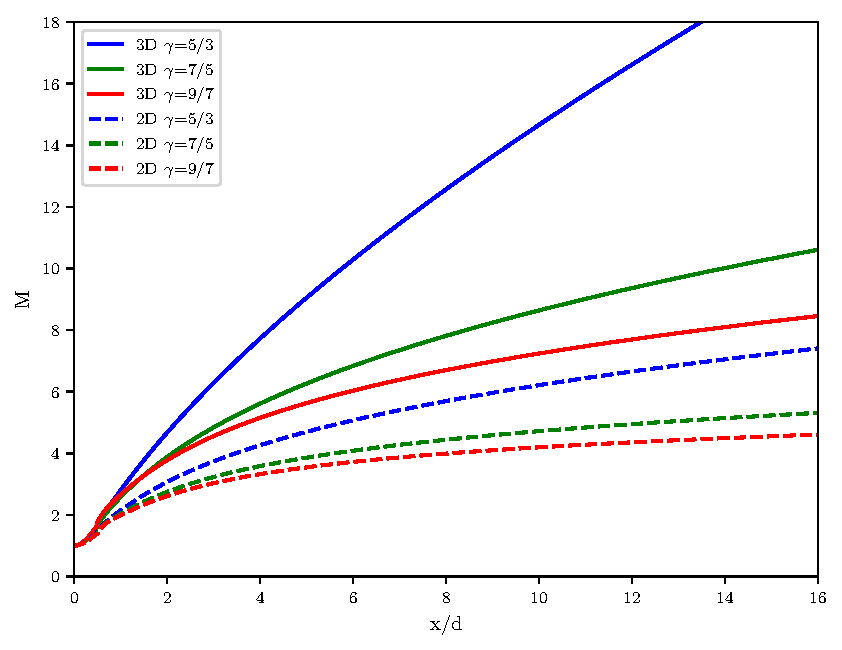
\includegraphics[width=0.5\textwidth]{figures/chap3/Scoles_Fig25.pdf}
%	\caption{Centerline Mach number versus distance in nozzle diameters for 2D (planar) and 3D (axisymmetric) geometries, calculated using \cref{eqn:Scoles_centerline2.2}.}
%	\label{fig:scoles_mach}
%\end{figure}
%
%\begin{figure}
%	\centering
%	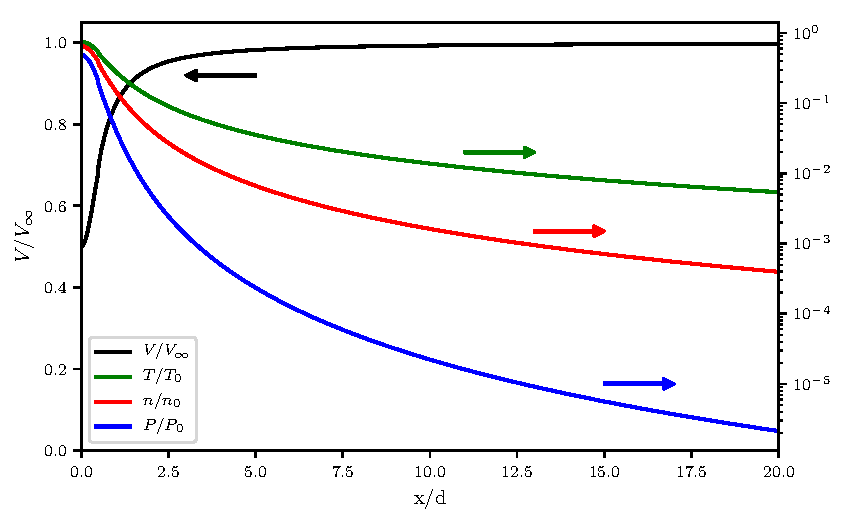
\includegraphics[width=0.5\textwidth]{figures/chap3/Scoles_Fig23.pdf}
%	\caption{Free jet centerline properties versus distance in nozzle diameters for helium gas ($\gamma$=5/3, W=4). Mach number is calculated using \cref{eqn:Scoles_centerline2.2}, and the centerline properties are calculated using \cref{eqn:mach_properties}. Velocity $V$ is scaled by terminal velocity $V_{\infty}$; temperature $T$, number density $n$ and pressure $P$ are normalized by source stagnation values $T_0$, $n_0$, $P_0$.}
%	\label{fig:scoles_centerline}
%\end{figure}

We use an \textit{in vacuo} gas nozzle to deliver a localized plume of gas near the IR focus. Generally, when gas flows from a high pressure region ($P_0$) to a low pressure region ($P_b$) through a small aperture of diameter $d$, a supersonic plume may form in the low pressure region. If the pressure ratio $P_0/P_b$ exceeds a critical value $G$, given by
\begin{equation}
G \equiv ((\gamma+1)/2)^{\gamma/(\gamma-1)} \le 2.1,
\label{eqn:G_factor}
\end{equation}
then the gas flow at the aperture will be equal to the speed of sound, and the pressure will be equal to $P_0 / G \approx P_0/2$. The highest chamber pressures in our experiments are on the order of $P_b \approx 10$ mTorr, and typical backing pressures for harmonic generation generally exceed 50 Torr, so we are always operating with a supersonic jet. The on-axis spatial extent of the supersonic gas plume is given by the Mach disk location, given by $x_M / d = 0.67 \sqrt{P_0/P_b}$. For a chamber pressure of 3 mTorr and a backing pressure of 450 Torr, $x_M = 260d = 51.9$ mm for a 200 $\mu$m diameter aperture. As will be shown below, our laser-gas interaction region is well within the structure of the gas jet.

The physics of supersonic gas flow have been discussed at length in the literature, so we will only go over the revelant highlights \cite{millerFreeJetSources1988}. The ratio of the velocity of the gas $V$ to the speed of sound $a$ is called the \textit{Mach number} $M=V/a$. It can be shown that all thermodynamic parameters within the supersonic structure (density, pressure, velocity and temperature) can be expressed in terms of the Mach number and the heat capacity ratio $\gamma$. For harmonic generation, we are primarily concerned with the on-axis ($y=0$) mass density $\rho$ and pressure $P$:
\begin{subequations}
	\label{eqn:mach_properties}
	\begin{align}
	\frac{\rho}{\rho_0} = \frac{n}{n_0} = \left(\frac{T}{T_0}\right)^{1/(\gamma-1)} &= \left(  1 + \frac{\gamma-1}{2} M^2 \right)^{-1/(\gamma-1)} \label{eqn:mach_rho} \\
	\frac{P}{P_0} = \left(\frac{T}{T_0}\right)^{\gamma/(\gamma-1)} &= \left(  1 + \frac{\gamma-1}{2} M^2 \right)^{-\gamma/(\gamma-1)} \label{eqn:mach_pressure}
	\end{align}
\end{subequations}
%\begin{align}
%\frac{\rho}{\rho_0} = \frac{n}{n_0} = \left(\frac{T}{T_0}\right)^{1/(\gamma-1)} &= \left(  1 + \frac{\gamma-1}{2} M^2 \right)^{-1/(\gamma-1)} \\
%\frac{P}{P_0} = \left(\frac{T}{T_0}\right)^{\gamma/(\gamma-1)} &= \left(  1 + \frac{\gamma-1}{2} M^2 \right)^{-\gamma/(\gamma-1)}
%\label{eqn:mach_properties}
%\end{align}
Here, $\rho_0$ is the mass density at the nozzle aperture ($x=0$), and $n$ is the number density. The Mach number is found by solving the fluid mechanics equations dealing with the conversation of mass, momentum and energy for a given nozzle geometry. For a complete discussion, see \cite{millerFreeJetSources1988}. Below we present the on-axis result, which is an analytic fit to a numerical solution of the thermodynamic equations:
\begin{subequations}
	\label{eqn:Scoles_centerline2.2}
	\begin{align}
	% eqns from table 2.2 of scoles, page 23
	\frac{x}{d} > 0.5&: &&M = \left( \frac{x}{d} \right)^{(\gamma-1)/j} \left[ C_1 + \frac{C_2}{\left(\frac{x}{d}\right)} + \frac{C_3}{\left(\frac{x}{d}\right)^2} + \frac{C_4}{\left(\frac{x}{d}\right)^3} \right] \label{eqn:Scoles_centerline1} \\
	0 < \frac{x}{d} < 1.0&: &&M = 1.0 + A \left( \frac{x}{d} \right)^2 + B \left( \frac{x}{d} \right)^3 \label{eqn:Scoles_centerline2}
	\end{align}
\end{subequations}
The fitting coefficients for \cref{eqn:Scoles_centerline2.2} are listed in \cref{tbl:Scoles_gas_params2.2}. We can see that $M$ scales with powers of $x/d$, the number of nozzle diameters away from the nozzle aperture. Likewise, the off-axis density $\rho(x,y)$ is given by:
\begin{align}
\frac{\rho(x,y)}{\rho(x,0)} &= \cos^2 \theta \cos^2 \left( \frac{\pi \theta}{2 \phi} \right) \\
\tan \theta &\equiv \frac{y}{x}
\label{eqn:off-axis-density}
\end{align}
where $y$ is the distance from the centerline axis, and $\phi$ is a gas constant with values ${\phi = 1.365, 1.662}$, and $1.888$ for ${\gamma = 5/3, 7/5}$ and $9/7$, respectively.

The gas nozzle throughput $\hat{T}$ is proportional to the area of the aperture and the backing pressure:
\begin{equation}
\hat{T} \ (\text{Torr} \cdot \text{l}/\text{s}) = C \left(\frac{T_C}{T_0} \right)\sqrt{\frac{300}{T_0}} P_0 d^2
\label{eqn:nozzle_thruput}
\end{equation}
where $C$ is a gas constant\footnote{Values of $C$ for common species are listed here: 45 [He], 20 [Ne], 14 [Ar], 16 [N\textsubscript{2}] l/cm\textsuperscript{2}/s. For a full table of values, see Table 2.5 in \cite{millerFreeJetSources1988}.}, $T_C$ and $T_0$ are the vacuum chamber and backing temperatures, respectively, and $d$ is the nozzle diameter in cm. Ignoring the effect of the generation chamber's vacuum aperture, we can estimate the operating pressure of the generation chamber using the following equation \cite{hablanianHighvacuumTechnologyPractical1997}:
\begin{equation}
P_b \ (\text{Torr}) = \frac{\hat{T}}{S}
\end{equation}
where $S$ is the pumping speed of the turbo pump. To avoid overloading our turbo pumps, we are  limited to operating pressures below 5 - 10 mTorr.

The basic design of our continuous free expansion nozzle is shown in \cref{fig:gas_nozzle}. The nozzle is an aluminum cylinder with a small diameter hole drilled into the top surface. Gas is delivered to the aperture via a universal gas receiver, which attaches to base of the nozzle. To reduce the gas load on the pumps, we used $200 \ \mu m$ diameter aperture, which was the smallest size hole the machine shop could readily drill into aluminum. A 200 $\mu$m diameter aperture backed with 180 Torr of argon will deliver a gas throughput of approximately {1 Torr $\cdot$ l/s}. With a pumping speed of $S = 1000$ L/s, the generation chamber pressure will be around $P_b = 1$ mTorr. For a monatomic gas, $G = 2.05$, and the pressure at the nozzle aperture is $P_0/G \approx 87 \textrm{ Torr}$.

The on-axis Mach number, density and pressure for a monoatomic gas are shown in \cref{fig:M_rho_vs_x}. We can see the on-axis gas density drops off precipitously with increasing distance from the nozzle $x$. Recalling \cref{fig:Constant1999_fig1}, we want to bring the nozzle as close to the optical axis to maximize the interaction density. However, if nozzle face enters the focal volume it will be drilled by the high intensity light and the resulting metallic plume will coat the generation chamber's vacuum window. Under normal operating conditions, we estimate the optical axis is located at $x=100 \ \mu$m. Using the numbers from our previous example, this gives us an argon interaction pressure of about 45 Torr and a number density of $2.67 \times 10^{24} \textrm{ m}^{-3}$.
% number density is calculated in \Python Scripts\HHG_Phasematching-master\test\Constant_fig1.py

The normalized off-axis gas density is shown in \cref{fig:off_axis_density}. At $x/d=0.5$, the FWHM of the density is $L_{med} = 120 \ \mu$m, which is smaller than the width of the laser spot size ($w_0 \sim 30 \ \mu$m), and the Rayleigh range ($z_R \sim 300 \ \mu$m).

We can now calculate the absorption length $L_{abs} = 1 / \rho \sigma$ for this jet. The photoabsorption cross section is relatively constant for argon in the range 45 - 150 eV \cite{gulliksonCXROXRayInteractions}. For argon at 100 eV, $\sigma = 2 r_0 \lambda f_2 = 1.3 \times 10^{-4} \textrm{ nm\textsuperscript{2}}$. Therefore the absorption length of the gas jet backed by 180 Torr of argon is $L_{abs} = 2.9 \textrm{ mm}$, and $L_{med}/L_{abs} = 0.04$. Referring back to \cref{fig:Constant1999_fig1,eqn:HHG_Nout_simple}, we can see that we are well within the quadratic regime of the HHG reabsorption model, regardless of the coherence length $L_{coh}$. Increasing the backing pressure by a factor of 5 will yield only $L_{med}/L_{abs} = 0.20$, still within the quadratic regime. This leaves significant room for HHG yield improvement.
% absorption length is calculated in \Python Scripts\HHG_Phasematching-master\test\Constant_fig1.py

%The structure of the resulting supersonic plume is shown in \cref{fig:gas_expansion}. The physics of supersonic gas flow has been extensively studied in the literature and will not be discussed at length here. Below is a brief overview of the relevant physics required to understand the gas nozzles used for HHG in our lab. For a more detailed review of the field, see Ref \cite{millerFreeJetSources1988}.

% derivation of \cref{eqn:gas_dens}
%energy equation. $V$ is velocity, $h$ is enthalpy per unit mass.
%\begin{equation}
%h + V^2/2 = h_0
%\end{equation}
%for ideal gases, $dh = \hat{C}_p \ dt$, and we have

%\begin{equation}
%V^2 = 2(h_0 -h) = 2 \int_{T}^{T_0} \hat{C}_p \ dT
%\label{eqn:Scoles_gas_jet_energy}
%\end{equation}

%For an ideal gas, $\hat{C}_p = \gamma / (\gamma-1) (R/W)$, where $\gamma = C_p/C_V$ is the ratio of the specific heats, $R$ is the gas constant, $W$ is the molecular weight. if the gas is cooled substantially in the expansion ($T \ll T_0$), then we have:

%\begin{equation}
%V_{\infty} = \sqrt{ \frac{2R}{W} \left( \frac{\gamma}{\gamma-1} \right) T_0 }
%\end{equation}

%For an ideal gas, the speed of sound is $a = \sqrt{\gamma R T/W}$ and the Mach number is $M = V/a$. Assuming $\hat{C}_p$ is constant, we can recast \cref{eqn:Scoles_gas_jet_energy} in terms of $\gamma$ and $M$.  Using these assumptions, one can obtain the following relationships for the temperature $T$, velocity $V$, pressure $P$, mass density $\rho$ and number density $n$ in the gas jet scaled to those parameters at the stagnation point $(T_0, P_0, \rho_0, n_0)$:

%\begin{subequations}
%	\label{eqn:mach_properties}
%	\begin{align}
%	% eqn 2.3 - 2.6 in scoles, page 18
%	(T/T_0) &= \left(  1 + \frac{\gamma-1}{2} M^2 \right)^{-1} \label{eqn:gas_temp} \\
%	V &= M \sqrt{ \frac{\gamma R T_0}{W} } \left( 1 + \frac{\gamma-1}{2} M^2 \right)^{-1/2} \label{eqn:gas_velo} \\
%	(P/P_0) &= (T/T_0)^{\gamma/(\gamma-1)} = \left(  1 + \frac{\gamma-1}{2} M^2 \right)^{-\gamma/(\gamma-1)} \label{eqn:gas_pres} \\
%	(\rho/\rho_0) &= (n/n_0) = (T/T_0)^{1/(\gamma-1)} = \left(  1 + \frac{\gamma-1}{2} M^2 \right)^{-1/(\gamma-1)} \label{eqn:gas_dens}
%	\end{align}
%\end{subequations}

%Therefore, once we know the Mach number $M$, we can calculate the above properties for the gas jet. The Mach number is found by solving the fluid mechanics equations dealing with the conversation of mass, momentum and energy:

%\begin{subequations}
%	\label{eqn:scoles_continuum}
%	\begin{flalign}
%	% eqn 2.7 of scoles, page 19
%	\text{mass:} && \nabla \cdot (\rho \mathbf{V}) &= 0 && \label{eqn:scoles_mass} \\
%	\text{momentum:} && \rho \mathbf{V} \cdot \nabla \mathbf{V} &= - \nabla P  && \label{eqn:scoles_momentum} \\
%	\text{energy:} && \mathbf{V} \cdot \nabla h_0 &= 0 \textrm{ or } h_0 = \textrm{constant along streamlines} \label{eqn:scoles_energy} && \\
%	\text{equation of state:} && P &= \rho \frac{R}{W} T  && \label{eqn:scoles_eqn-state} \\
%	\text{thermal equation of state:} && dh &= \hat{C}_P \ dT \label{eqn:scoles_thermal-eqn-state} && 
%	\end{flalign}
%\end{subequations}

%The above equations are valid for an isentropic, compressible flow of a single component ideal gas molecular weight $W$ and constant specific heat ratio $\gamma$. A steady state is assumed and viscosity and heat conduction are neglected. These equations have been numerically solved in the literature for two source geometries: a ``slit" nozzle (2D, planar) and a circular aperture (3D, axisymmetric). The numerical solutions to each geometry scale with the nozzle diameter $d$, and have been fit to the following analytical functions:

%\begin{subequations}
%	\label{eqn:Scoles_centerline2.2}
%	\begin{align}
%	% eqns from table 2.2 of scoles, page 23
%	\frac{x}{d} > 0.5&: &&M = \left( \frac{x}{d} \right)^{(\gamma-1)/j} \left[ C_1 + \frac{C_2}{\left(\frac{x}{d}\right)} + \frac{C_3}{\left(\frac{x}{d}\right)^2} + \frac{C_4}{\left(\frac{x}{d}\right)^3} \right] \label{eqn:Scoles_centerline1} \\
%	0 < \frac{x}{d} < 1.0&: &&M = 1.0 + A \left( \frac{x}{d} \right)^2 + B \left( \frac{x}{d} \right)^3 \label{eqn:Scoles_centerline2}
%	\end{align}
%\end{subequations}

%\textbf{question: why does M increase without bound with increasing x, while V is limited to a finite value? scoles has a discussion, you should address it here.}

%The fitting coefficients for \cref{eqn:Scoles_centerline2.2} are listed in \cref{tbl:Scoles_gas_params2.2}. A plot of the results for different source geometries and gases are shown in \cref{fig:scoles_mach}.





%\cref{tbl:Scoles_mach_params} shows the centerline Mach numbers used in the following equations:

%\begin{subequations}
%	\label{eqn:Scoles_centerline2.1}
%	% eqns from table 2.1 of scoles, page 22
%	\begin{align}
%	M &= A \left( \frac{x-x_0}{d}\right)^{\gamma-1} - \frac{\frac{1}{2} \left( \frac{\gamma+1}{\gamma-1} \right)}{A \left(\frac{x-x_0}{d} \right)^{\gamma-1}} \label{eqn:gas_mach} \\
%	\frac{\rho(y,x)}{\rho(0,x)} &= \cos^2(\theta) \cos^2\left(\frac{\pi\theta}{2\phi}\right) \\
%	\frac{\rho(R,\theta)}{\rho(R,0)} &= \cos^2\left(\frac{\pi\theta}{2\phi}\right) \\
%	\left(\frac{x}{d} \right) &> \left( \frac{x}{d} \right)_{\text{min}} \label{eqn:mach_cond}
%	\end{align}
%\end{subequations}
%The gas nozzle throughput $\hat{T}$ is calculated from:
%\begin{equation}
%\hat{T} \ (\text{torr} \cdot \text{l}/\text{s}) = \hat{S} \cdot P_b = C \left(\frac{T_C}{T_0} \right)\sqrt{\frac{300}{T_0}}(P_0 d) d
%\label{eqn:nozzle_thruput}
%\end{equation}

%where $C$ is the gas constant from \cref{tbl:Scoles_gas_params}, $P_0$ is the nozzle's backing pressure in Torr, $T_C$ and $T_0$ are the vacuum chamber and backing temperatures, respectively, in Kelvin, $P_0$ is the backing pressure in Torr, and $d$ is the nozzle's diameter in cm.

%
%\begin{table}[]
%	\centering
%	\begin{tabular}{llllll}
%		Gas    & $\epsilon / k$ (K) & $\sigma$ (angstrom) & $C_6 / k$ ($10^{-43}$ K $\cdot$ cm$^6$) & $Z_r$     & \begin{tabular}[c]{@{}l@{}}C (l/cm$^2$/s);\\ \cref{eqn:nozzle_thruput}\end{tabular} \\ \hline
%		He     & 10.9               & 2.66                & 0.154                                   & -         & 45                                                               \\
%		Ne     & 43.8               & 2.75                & 0.758                                   & -         & 20                                                               \\
%		Ar     & 144.4              & 3.33                & 7.88                                    & -         & 14                                                               \\
%		Kr     & 190                & 3.59                & 16.3                                    & -         & 9.8                                                              \\
%		Xe     & 163                & 4.3                 & 41.2                                    & -         & 7.9                                                              \\
%		H$_2$  & 39.6               & 2.76                & 0.7                                     & $\sim$300 & 60-63                                                            \\
%		D$_2$  & 35.2               & 2.95                & 0.93                                    & $\sim$200 & 42                                                               \\
%		N$_2$  & 47.6               & 3.85                & 6.2                                     & $\sim$2.5 & 16                                                               \\
%		CO     & 32.8               & 3.92                & 4.76                                    & $\sim$4.5 & 16                                                               \\
%		CO$_2$ & 190                & 4.0                 & 31.1                                    & $\sim$2.5 & 12-13                                                            \\
%		CH$_4$ & 148                & 3.81                & 18.1                                    & $\sim$15  & 21                                                               \\
%		O$_2$  & 115                & 3.49                & 8.31                                    & $\sim$2   & 15                                                               \\
%		F$_2$  & 121                & 3.6                 & 10.5                                    & $\sim$3.5 & 14                                                               \\
%		I$_2$  & 550                & 4.98                & 336                                     & $\sim$1   & 5.2                                                              \\ \hline
%	\end{tabular}
%	\caption{Gas parameters used in free expansion calculations. Table recreated from Ref \cite{millerFreeJetSources1988}.}
%	\label{tbl:Scoles_gas_params2.1}
%\end{table}
%
%\begin{table}[]
%	\centering
%	\begin{tabular}{lllll}
%		\hline
%		$\gamma$ & $x_0/d$ & $A$  & $\phi$ & $(x/d)_{\text{min}}$ \\ \hline
%		1.67     & 0.075   & 3.26 & 1.365  & 2.5                  \\
%		1.40     & 0.4     & 3.65 & 1.662  & 6                    \\
%		1.2857   & 0.85    & 3.96 & 1.888  & 4                    \\
%		1.20     & 1.00    & 4.29 & -      & -                    \\
%		1.10     & 1.60    & 5.25 & -      & -                    \\
%		1.05     & 1.80    & 6.44 & -      & -                    \\ \hline
%	\end{tabular}
%	\caption{Centerline Mach Number and Off-Axis Density Correlations for Axisymmetric Flow. Table recreated from Ref \cite{millerFreeJetSources1988}.}
%	\label{tbl:Scoles_mach_params}
%\end{table}

\subsection{Low Pressure Cell}

\begin{figure}
	\centering
	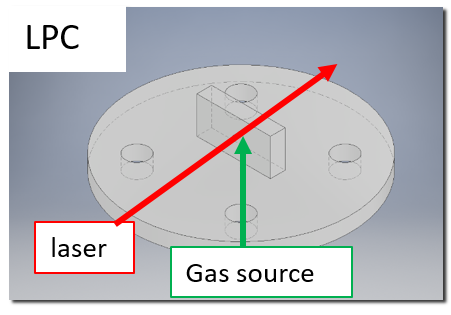
\includegraphics[width=0.5\textwidth]{figures/chap3/LPC_diagram.png}
	\caption{Rendering of the low pressure cell (LPC).}
	\label{fig:LPC_diagram}
	% figure created in Chap 3 figures powerpoint.
\end{figure}

The interaction region of the free expansion nozzle would have much higher pressures if the laser could be sent down the symmetry axis of the gas plume, but this is not possible given the nozzle's geometry. The low pressure cell (LPC), shown in \cref{fig:LPC_diagram}, was designed to solve this problem.\footnote{Special thanks to Zhou Wang \cite{wangMidinfraredStrongfieldLaser2018} for designing the original LPC. The LPC used in this work has been slightly modified to work with our universal gas receiver.} The LPC consists of an aluminum disk with rectangular block at the center of the top surface. Gas flows from the universal gas receiver (which is mated to the bottom of the disk) through a thin capillary and into the rectangular block. A through hole drilled into the front face of the rectangular block intersects the capillary and serves as the gas-laser interaction volume. Below, we will model the gas density profile of the LPC and show that the thickness of the block ($W = 2.032$ mm) sets the gas-laser interaction length.

\subsubsection{Calculating the Interaction Pressure}

\begin{figure}
	\centering
	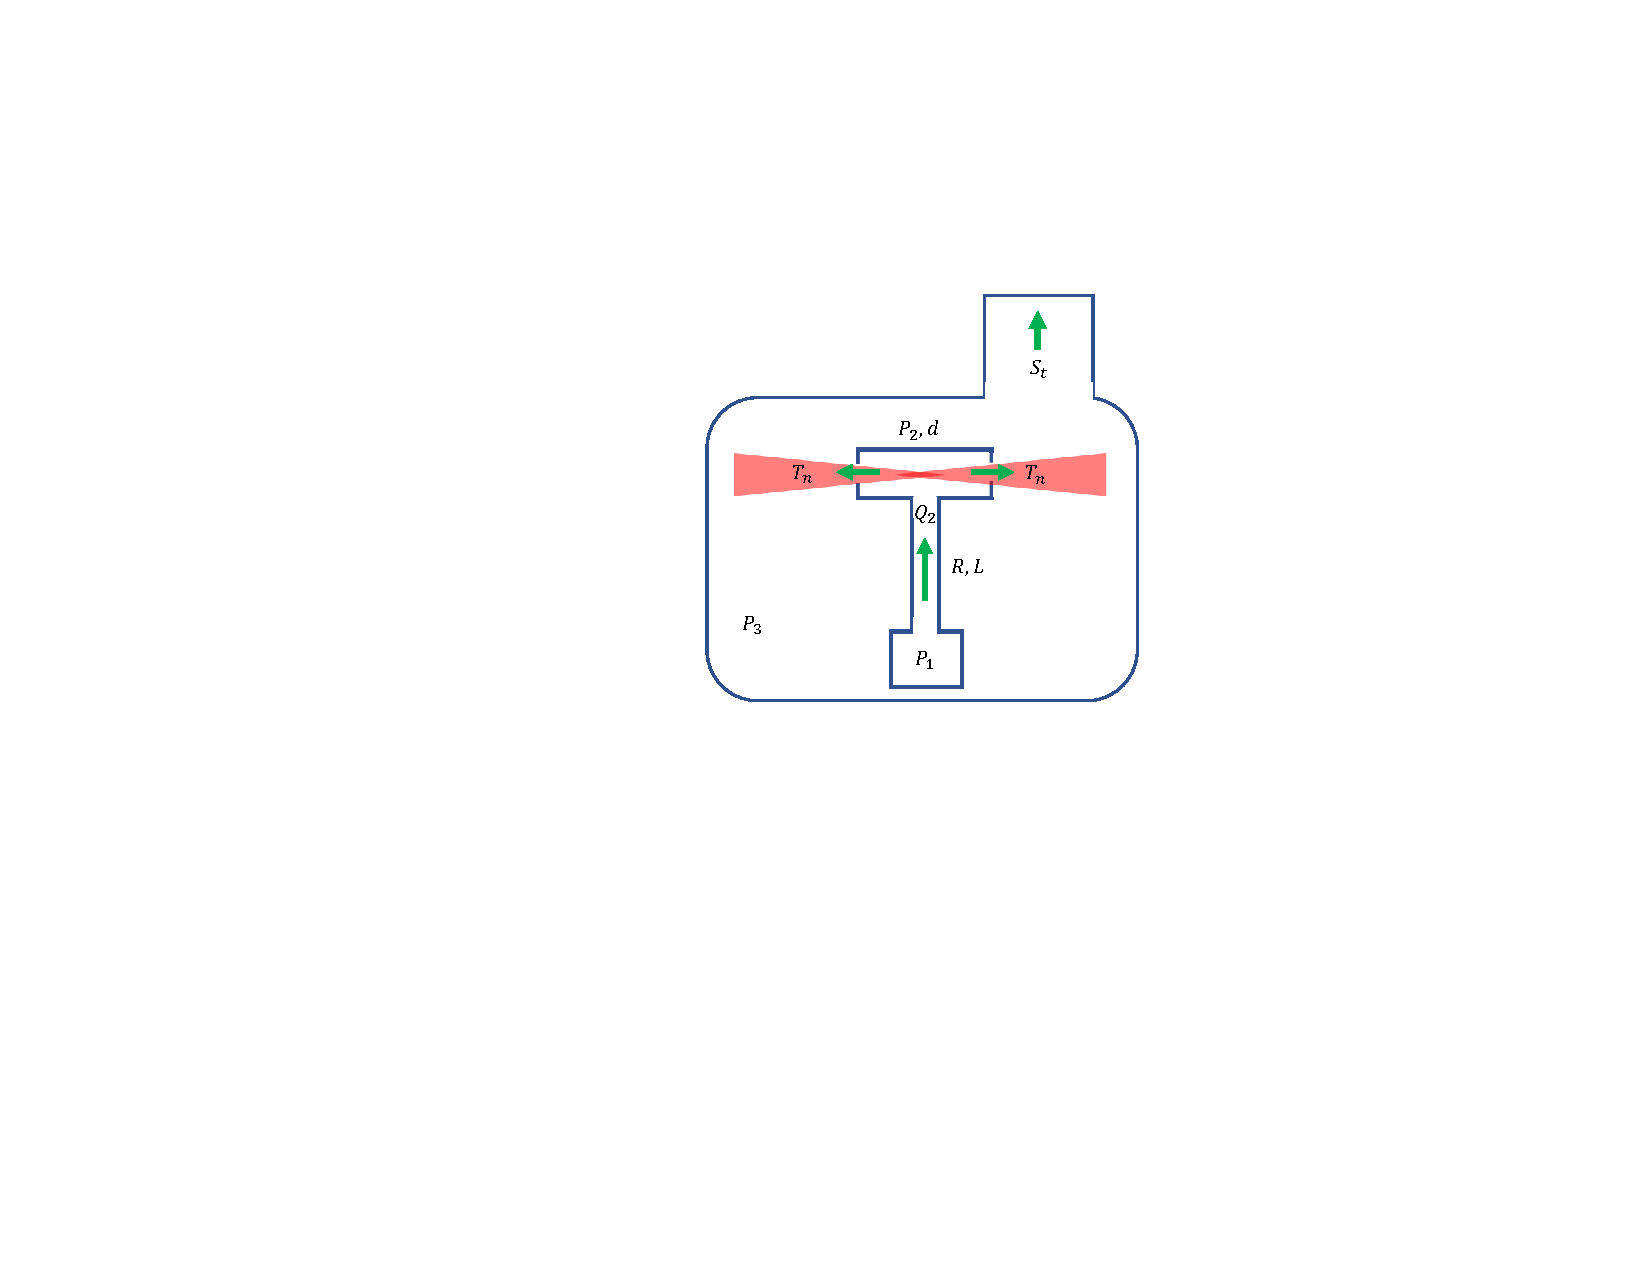
\includegraphics[width=0.75\textwidth]{figures/chap3/LPC_schematic.pdf}
	\caption{Gas flow schematic of the LPC.}
	\label{fig:LPC_schematic}
	% figure created in Chap 3 figures powerpoint.
\end{figure}

\begin{figure}
	\centering
	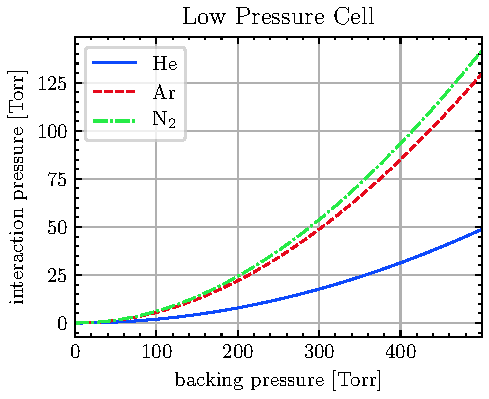
\includegraphics[width=0.75\textwidth]{figures/chap3/LPC_interaction_p.pdf}
	\caption{Calculated pressure in the LPC interaction region.}
	\label{fig:LPC_interaction_p}
	% figure created in \Python Scripts\HPC\HPCvsLPC.py
\end{figure}

\begin{figure}
	\centering
	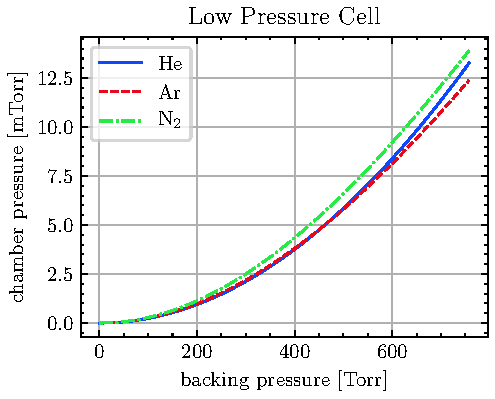
\includegraphics[width=0.75\textwidth]{figures/chap3/LPC_chamber_p.pdf}
	\caption{Calculated pressure in the target chamber using the LPC.}
	\label{fig:LPC_chamber_p}
	% figure created in \Python Scripts\HPC\HPCvsLPC.py
\end{figure}

\begin{figure}
	\centering
	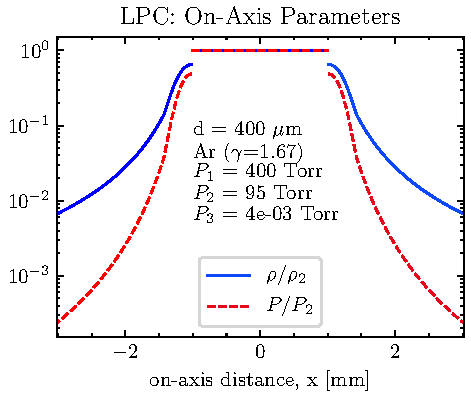
\includegraphics[width=0.75\textwidth]{figures/chap3/LPC_on_axis.pdf}
	\caption{On-axis density and pressure for the low pressure cell.}
	\label{fig:LPC_on_axis}
	% figure created in \Python Scripts\HPC\HPCvsLPC.py
\end{figure}

\cref{fig:LPC_schematic} shows a gas flow model of the LPC. The green arrows indicate the direction of gas flow, and the red shaded region indicates the laser focus. The gas receiver is considered to be an infinite reservoir of gas with pressure $P_1$. This region supplies the laser interaction region with gas via a thin capillary of diameter $R = 101.5 \ \mu \textrm{m}$, length $L = 5 \textrm{ mm}$ and volumetric flow rate $Q_2$, modelled as an ideal isothermal gas \cite{fryerTheoryGasFlow1966,venerusLaminarCapillaryFlow2006,landauFluidMechanics2011}. The interaction region with pressure $P_2$ acts as a pressure source for two diametrically opposed supersonic gas jets \cite{millerFreeJetSources1988}, each with diameter $d = 400 \ \mu \textrm{m}$ and throughput $\hat{T}_{n}$. The generation chamber has a turbopump with pumping speed $S_{t}$ and an equilibrium pressure $P_3$. This results in the following coupled equations (SI units):
\begin{align}
p_1^2 - p_2^2 &= \frac{16 \mu L Q_2 p_2}{\pi R^4} \\
Q_2 p_2 &= 2 T_n \\
p_3 &= \frac{2 \hat{T}_n}{S_t} \\
\hat{T}_n &= c p_2 d^2
\label{eqn:LPC_coupled_equations}
\end{align}
where $c$ is a gas constant expressed in \si{m/s} (see \cref{eqn:nozzle_thruput}) and $\mu$ is the dynamic viscosity in \si{Pa.s}. Solving for the interaction pressure $p_2$ and chamber pressure $p_3$, we obtain:
\begin{align}
p_2 &= - \frac{16 c d^2 L \mu}{\pi R^4} + \sqrt{p_1^2 + \frac{256 c^2 d^4 L^2 \mu^2}{\pi^2 R^8}} \\
p_3 &= \frac{2 c d^2}{S_t} \left( - \frac{16 c d^2 L \mu}{\pi R^4} + \sqrt{p_1^2 + \frac{256 c^2 d^4 L^2 \mu^2}{\pi^2 R^8}}  \right)
\label{eqn:LPC_pressures}
\end{align}
These functions are shown in \cref{fig:LPC_interaction_p,fig:LPC_chamber_p}. Experimentally, we are limited to backing pressures of about 400 Torr or less in the LPC, which yields interaction pressures below 100 Torr for argon or nitrogen, and below 30 Torr in helium. Somewhat counterintuitively, the interaction pressure is lower for helium than the other species for a given backing pressure. This is because helium has a larger value of $c$ that prevents it from being trapped in the interaction region. 

\cref{eqn:mach_properties} can be used to calculate the on-axis density and pressure of the LPC, which are shown in \cref{fig:LPC_on_axis}. Note that due to the $G$ factor (\cref{eqn:G_factor}), the FWHM of the pressure and density is simply the width of the LPC's rectangular block: $L_{med} = 2.032$ mm. Due to the negligible gas density outside of the interaction region, we will treat the gas density as a boxcar function with a thickness $L_{med} = 2.032 \textrm{ mm}}$ set by dimensions of the rectangular block.

%Labs calculations done in \Python Scripts\HHG_Phasematching-master\test\Constant_fig1.py
When operating at maximum backing pressure, the maximum absorption length for the LPC at 100 eV in argon is identical to that of the free expansion jet: $L_{abs} = 0.6 \ \textrm{mm}$. However, the longer interaction length of the LPC yields a much higher ratio $L_{med}/L_{abs} = 3.5$.

justification for treating the gas thru hole as two diametrically opposed gas jets. compare the mean free path of $p_2$ region to the thickness of the rectangular block. note that we are in the supersonic regime, since p2 is more than 2x p3.

\subsubsection{HHG in LPC}

\begin{figure}
	\centering
	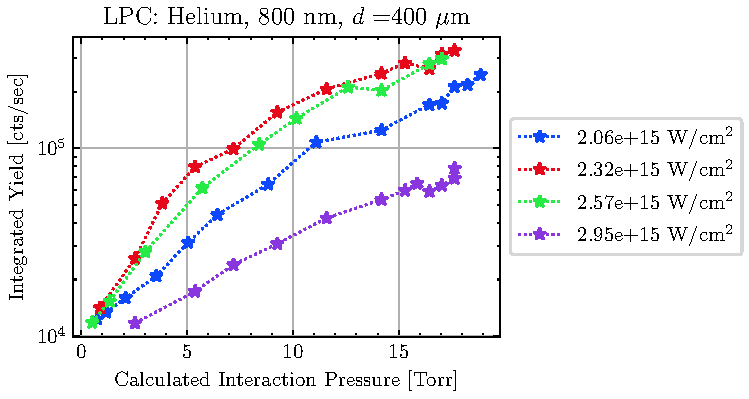
\includegraphics[width=0.75\textwidth]{figures/chap3/LPC_P_scaling_He800.pdf}
	\caption{Total harmonic yield of the LPC as a function of interaction pressure.}
	\label{fig:LPC_performance}
	% figure created in Python Scripts\HPC\LPC_800nm.py
\end{figure}

\textbf{compute absorption length, Lmed/Labs for helium}





\cref{fig:LPC_performance} shows the pressure scaling of the LPC when using an 800 nm pulse and helium gas. The interaction pressure is calculated from the backing pressure and the geometry of the nozzle using \cref{eqn:LPC_pressures}. From this figure, we can see that the harmonic yield increases with increasing interaction pressure. Using the 1D model of \cref{sec:XUV_reabsorption}, this trend indicates that we are operating in a sub-optimal interaction geometry, and increasing the pressure-length would improve our harmonic yield.

\cref{fig:HHG-HPCvsLPCHPC} shows a spectrum using optimized generation conditions (17 Torr interaction pressure, 1.85 mJ). Under these conditions, the highest resolvable harmonic is at 104 eV. From \cref{eqn:cutoff_energy}, we estimate $U_p = 25 \textrm{ eV}$ and $I_0 = 4.2 \times 10^{14} \textrm{ W/cm\textsuperscript{2}}$. On the other hand, if we calculate the peak intensity from the input pulse energy, we would expect $I_0 = 6 \times 10^{15} \textrm{ W/cm\textsuperscript{2}}$, nearly an order of magnitude higher that the HHG spectrum suggests. This suggest an inability to phase match the high energy photons.

Under these conditions, with a 400 mm focal length, we estimate the interaction energy to be $6 \times 10^{15}$ W/cm\textsuperscript{2}, and $U_p = $ From \cref{eqn:Up,eqn:cutoff_energy}, we calculate 




can you predict the cutoff energy using the interaction intensity? for a cutoff energy of 100 eV, at 800 nm, in helium (assuming perfect phase matching), Up = 23.78 eV, and I = $4 \times 10^{14}$ W/cm\textsuperscript{2}. do we have perfect phase matching?

calculate the interaction intensity from the input beam. assuming a 16 mm diameter beam, 1.89 W of input power at 800nm, we should have an intensity of $1 \times 10^{16}$ W/cm\textsuperscript{2}, which is 25 times higher than the intensity predicted from the cutoff energy. if we had this intensity, our cutoff would be way higher ... something's not right. maybe we just can't phase match the higher photon energies? 



advantages: increased interaction length - brighter! easy to align.

disadvantages: relative to the free expansion nozzle, you don't get any cooling.

\subsection{High Pressure Cell}
\label{sec:HPC}

\begin{figure}
	\centering
	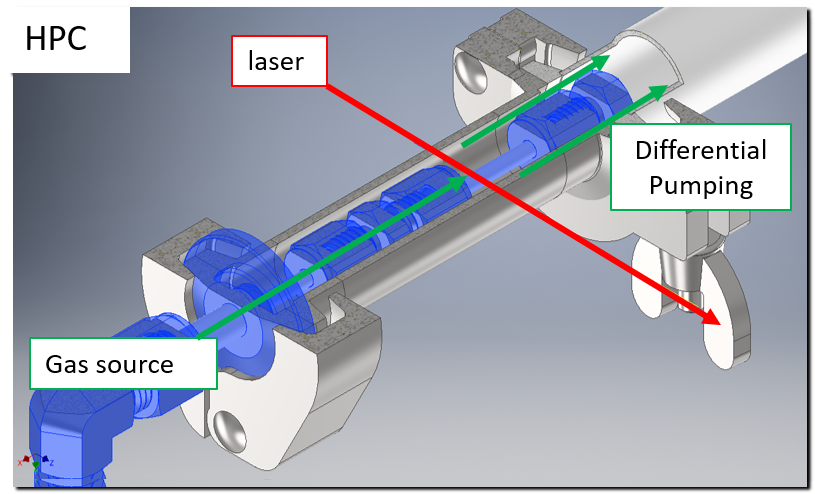
\includegraphics[width=0.75\textwidth]{figures/chap3/HPC_cutaway2.png}
	\caption{Cutaway view of the HPC interaction region. From bottom left to top right: welded gas feedthrough, concentric inner \& outer pipes, connection to edge-welded bellows. The high pressure region is shaded blue. The green lines indicate the gas flow direction; the red line indicates the laser propagation direction.}
	\label{fig:HPC_cutaway2}
\end{figure}

\begin{figure}
	\centering
	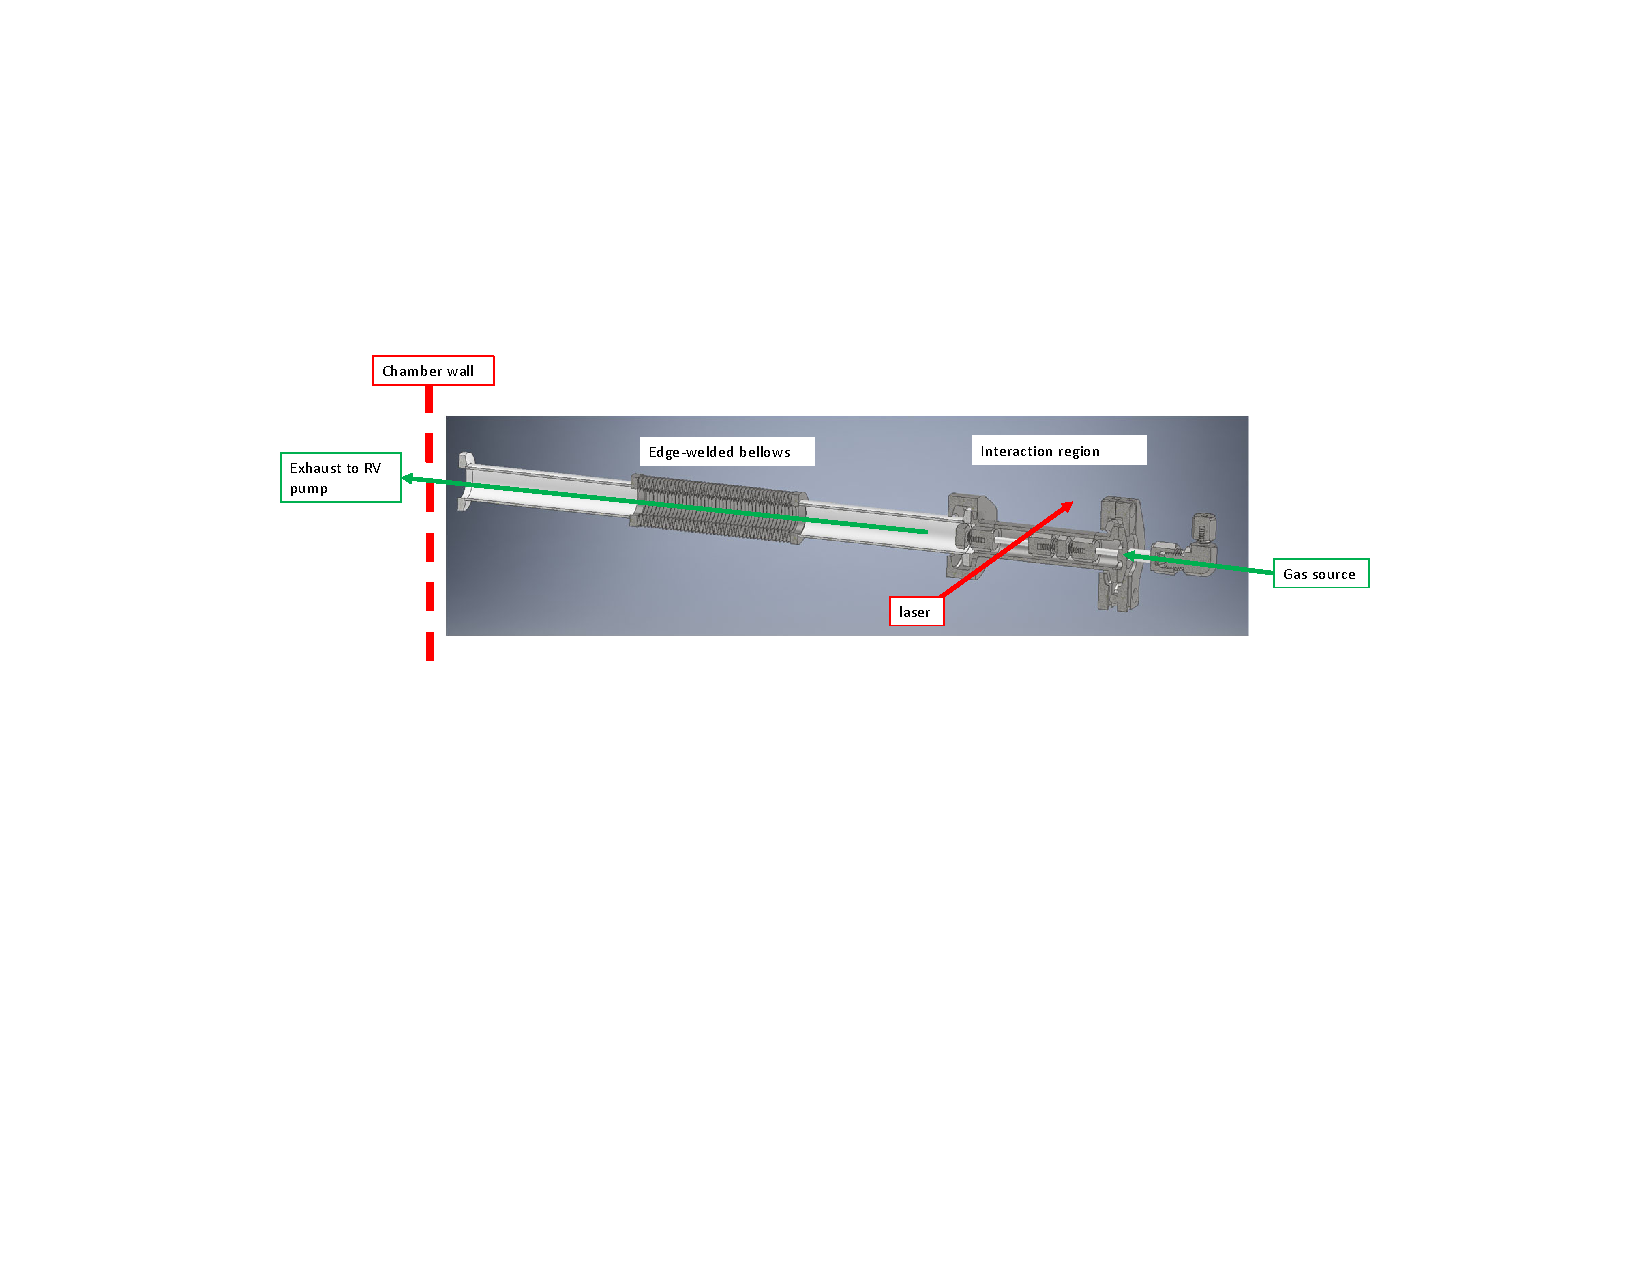
\includegraphics[width=1.0\textwidth]{figures/chap3/HPC_cutaway_bellows.pdf}
	\caption{Cutaway view of the HPC assembly showing the flexible bellows connection and connection to the chamber wall.}
	\label{fig:HPC_cutaway_bellows}
\end{figure}

\begin{figure}
	\centering
	
\includegraphics[width=0.5\textwidth]{figures/chap3/HPC_laserhole_500x370.png}
	\caption{Photograph of the HPC's inner pipe showing the laser-drilled hole (bottom center of pipe). See text for details.}
	\label{fig:HPC_laserhole}
	% pictures of the HPC inner holes are located in \OneDrive - The Ohio State University\DiMauro\lab pics\HPC. The original TIFF picture was cropped with GIMP, then downsized and exported as a png.
\end{figure}


\subsubsection{Design of HPC}

The high pressure cell (HPC) was designed to be a drop-in upgrade to the previously available HHG gas sources. As such, we did not consider a semi-infinite gas cell design which would require disruptive chamber modifications. We also did not want to implement a waveguide solution, as its performance would be strongly effected by the coupling (and therefore the laser pointing) into the assembly \cite{popmintchevExtendedPhaseMatching2008,popmintchevPhaseMatchingHigh2009}. Finally, we wanted to avoid the complications of a pulsed solenoid valve \cite{evenEvenLavieValveSource2015}, so the HPC was designed to be user-servicable with low-cost replacement parts. As such, it consists of standard Swagelok and KF fittings with minimal modifications and a custom bellows assembly. The only consumable part is the stainless steel pipe housing the interaction region, and it only needs to be replaced when the HPC is installed or the focusing condition is changed.

The design of the HPC is shown in \cref{fig:HPC_cutaway2,fig:HPC_cutaway_bellows}. It features two concentric cylinders: a stainless steel inner pipe which serves as the interaction region and gas source, and an outer shroud connected to an external rough pump which provides differential pumping. The inner pipe is connected to a gas line with continous flow. Laser-drilled diametrically opposed pinholes on the inner pipe wall allow for light propagation while minimizing gas flow to the outer shroud. A small portion of the gas within the outer shroud flows into the generation chamber via the machined holes, but most of the gas flows towards the exhaust and into a dedicated rough pump.

The relative positions of the inner pipe and the outer shroud are fixed by the KF hardware connections upon assembly. However, this positioning is not repeatable within the tolerances imposed by the laser transmission requirements. As a result, a new section of stainless steel pipe must be laser drilled every time the HPC is disassembled or removed from the generation chamber. The HPC assembly's position relative to the laser is adjustable via the same vacuum XYZ manipulator. A set of flexible bellows, visible in \cref{fig:HPC_cutaway_bellows}, allows for this movement while maintaining a vacuum-tight connection between the outer shroud and the chamber wall. A Baratron pressure gauge monitors the pressure inside the bellows and the outer shroud during operation.\footnote{Note: the bellows cannot withstand an internal pressure differential greater than 120 Torr. See \cref{app:HPC_instructions} before operating this system.} The flexible bellows has enough slack to allow the HPC to move below the optical axis, allowing the beam to pass over the top of the outer shroud. This is useful when aligning downstream optics.

The laser passes through the HPC assembly perpendicular to its symmetry axis; therefore the gas-laser interaction length is approximately equal to the diameter of the inner pipe. The outer shroud has two diametrically opposed machined 600 $\mu$m holes for the laser to pass through the assembly. During installation, the user aligns the two apertures in the outer shroud to the laser and fixes its position. Next, the inner pipe is installed and the unattentuated laser drills through the inner pipe walls. Therefore, the four apertures are automatically colinear and aligned to the laser propagation axis.

\cref{fig:HPC_laserhole} shows a photograph of the laser-drilled holes, taken with a 0.5x telecentric lens (Edmund Optics part number 62-911). Laser drift \&  misalignment, as well as daily harmonic optimization procedures over the course of several months have opened up these holes from their original diameter of approximately $100 \ \mu \textrm{m}$ to a final diameter of $430 \ \mu \textrm{m}$.

\subsubsection{Gas Flow in HPC}

\begin{figure}
	\centering
	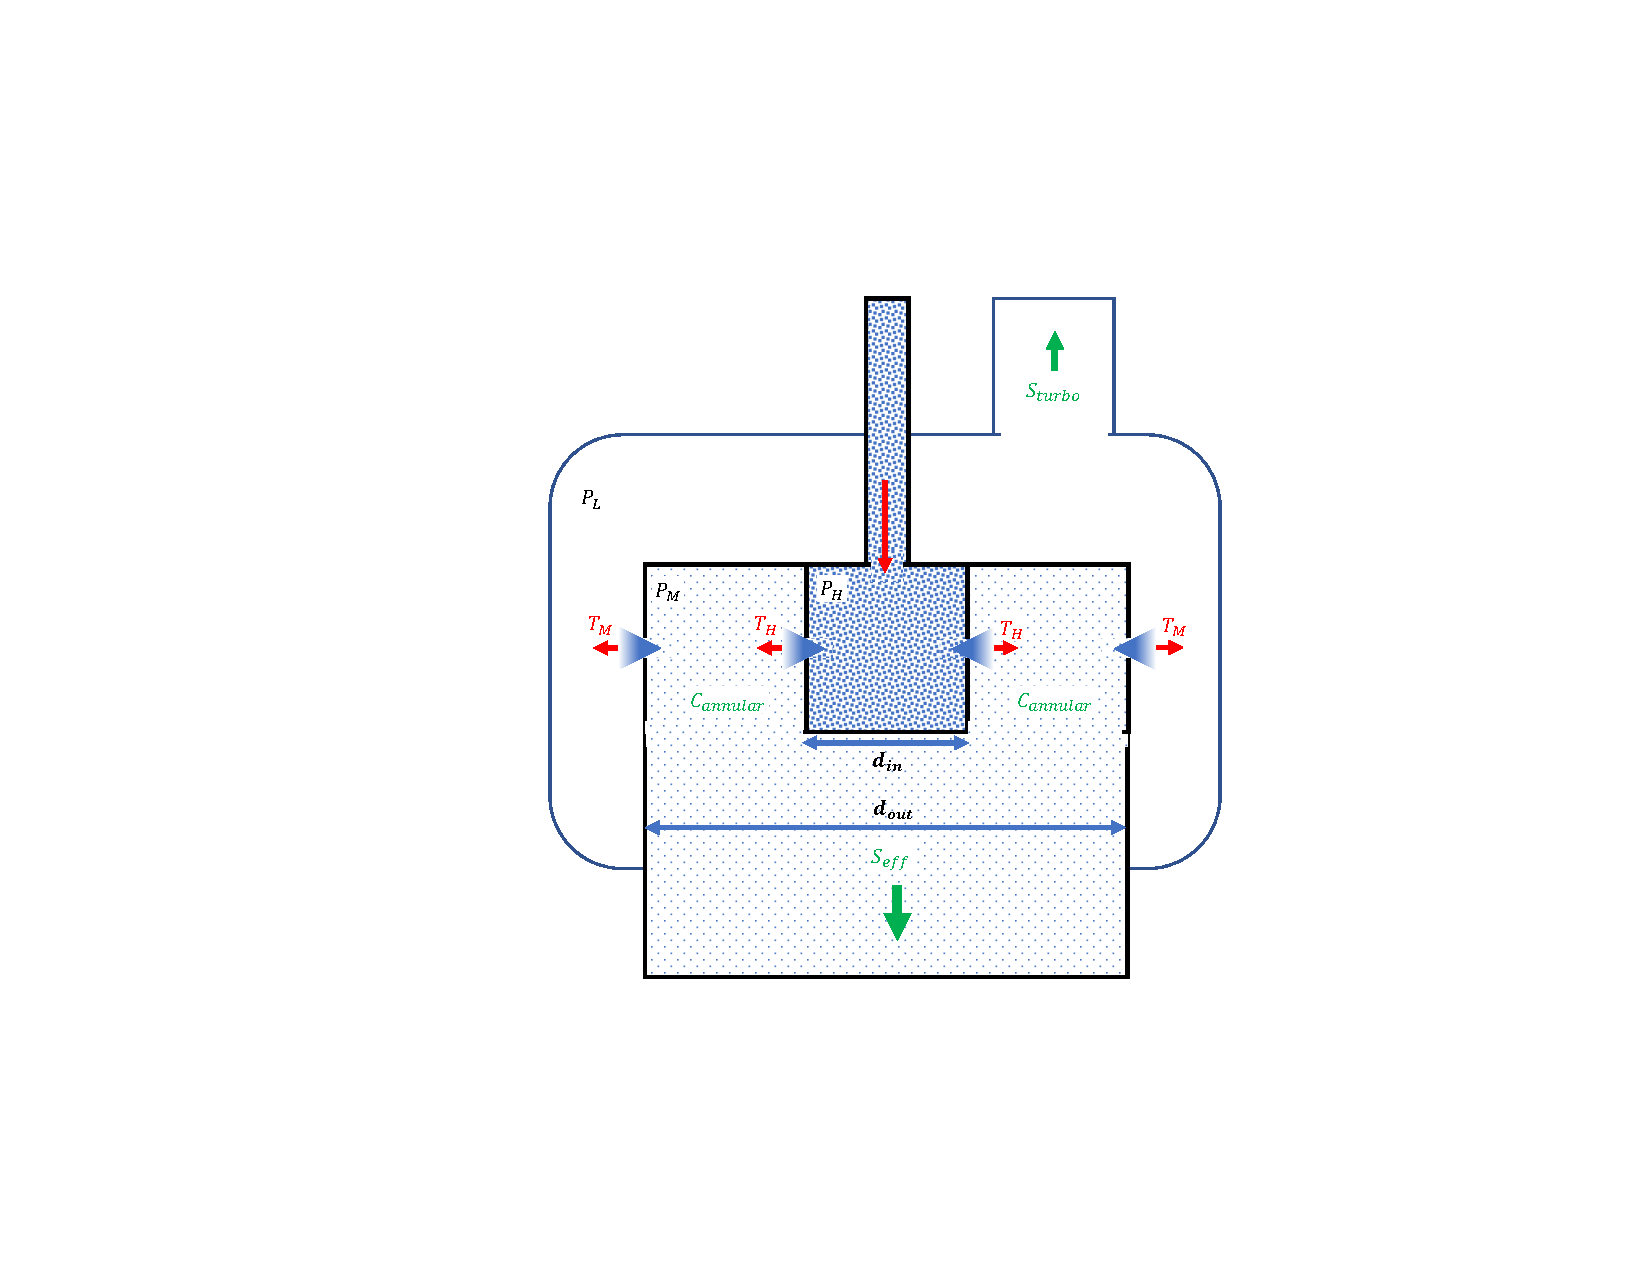
\includegraphics[width=0.75\textwidth]{figures/chap3/HPC_pressure_schematic.pdf}
	\caption{Schematic used to calculate the pressures inside the HPC and generation chamber.}
	\label{fig:HPC_pressure_schematic}
	% chap3 powerpoint
\end{figure}

\begin{figure}
	\centering
	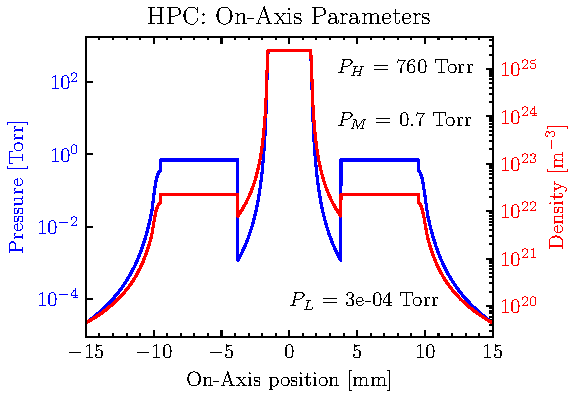
\includegraphics[width=0.75\textwidth]{figures/chap3/HPC_on-axis-pressure.pdf}
	\caption{Calculated on-axis pressure in the HPC for argon with $P_H = 760$ Torr, $P_M = 3$ Torr and $P_L = 3 \times 10^{-4}$ Torr.}
	\label{fig:HPC_on-axis-pressure}
	% plot made in \Python Scripts\HPC\HPCvsLPC.py
\end{figure}

\begin{figure}
	\centering
	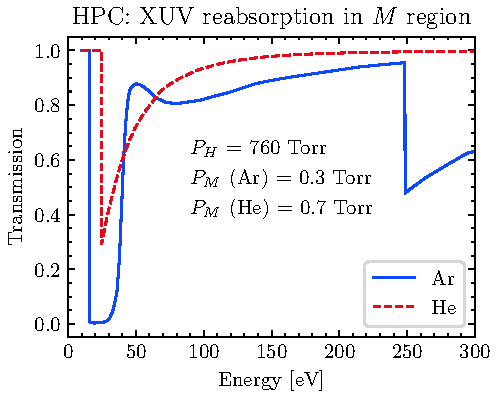
\includegraphics[width=0.75\textwidth]{figures/chap3/HPC_absorption.pdf}
	\caption{XUV reabsorption in the $P_M$ region for different generating media.}
	\label{fig:HPC_absorption}
	% plot made in \Python Scripts\CXRO\test\CXRO.py
\end{figure}

The geometry of the HPC assembly allows the user to use much higher interaction pressures than other continuous gas sources in the DiMauro lab. Here, we will model the gas flow through the HPC to see why this is the case. \cref{fig:HPC_pressure_schematic} shows the gas flow and relevant geometry. With the HPC cell installed, there are three distinct pressure regions: the high pressure inner pipe, the medium pressure outer shroud, and the low pressure generation chamber. Gas flows from the high pressure region through the laser drilled apertures into the medium pressure region. In the medium pressure region, gas flows through the machined apertures on the outer shroud's walls into the vacuum chamber, or down the bellows assembly to the rough pump.

We define the relevant variables in \cref{fig:HPC_pressure_schematic}. The dark blue region represents the high pressure region ($P_H$), the light blue region represents the medium pressure region ($P_M$), and the low pressure region is represented by the white region ($P_L$). Red arrows and text indicate gas sources, green arrows and text indicate flow towards the vacuum pumps; blue arrows and text indicate physical dimensions. $P_H$, $P_M$, and $P_L$ are the pressures of the inner pipe, outer shroud, and generation chamber, respectively; $S_{turbo}$, $S_{eff}$ and $C_{annular}$ are the turbo pumping speed, effective rough pumping speed and annular conductance, respectively; $T_H$ ($T_M$) is the gas throughput from the high (medium) pressure region into the medium (low) pressure region.

We assume that the high pressure region is an infinite gas reservoir held at pressure $P_H$ set by the regulator on the gas cylinder. The medium pressure region has a net gas throughput of $Q_M = 2(T_H - T_M)$ and an effective pumping speed $S_{eff}$. The low pressure region has a gas throughput of $2T_M$ and a pumping speed of $S_{turbo}$. The pressure in each region is simply $P = Q / S$. Owing to the large pressure differentials between adjacent regions, the gas throughput of the apertures is supersonic and is proportional to the area of the aperture and the backing pressure, following \cref{eqn:nozzle_thruput}:
\begin{equation}
T_H = c P_H a_H^2,
\end{equation}
where $a_H$ is the diameter of the laser drilled aperture. The supersonic expansion gives rise to a plume structure with an on-axis spatial extent given by the Mach disk location, $x_M / a_H = 0.67 \sqrt{P_H/P_M}$ \cite{millerFreeJetSources1988}. At on-axis distances larger than $x_M$, we can ignore the supersonic plume structure and consider only the background pressure $P_M$. For $P_H = 760$ Torr, $P_M = 3$ Torr and $a_H = 100 \ \mu$m, $x_M = 10.6 a_H = 1.06$ mm. Since the distance between the laser drilled aperture and the outer shroud's machined hole (6.2825 mm) is much greater than $x_M$, so we can ignore the supersonic plume structure when considering the gas flow from the medium pressure region to the low pressure region. As a result, $T_M$ has the same form as $T_H$:
\begin{equation}
T_M = c P_M a_M^2
\end{equation}
We can calculate the Mach disk location for the machined apertures using measured pressures in each region: for $P_M = 3$ Torr, $P_L = 3 \times 10^{-4}$ Torr, and $a_M = 600 \ \mu$m, we have $x_M = 67 a_M = 40.2$ mm. This distance is much smaller than the distance between the HPC and the next vacuum chamber (25 cm), so we can ignore the effect of the HPC's supersonic plumes on the rest of the beamline.

The medium pressure region is pumped by a small RV pump with pumping speed $S_{RV}$. This pumping speed is reduced by the geometry of the pipes between the shroud's apertures and the mouth of the pump. First, the inner pipe and outer shroud form an annual pipe; secondly, the bellows and the several feet of soft PVC tubing further reduce the pumping speed. Given the relatively high pressures in the medium pressure region (a few Torr), the mean free path of the gas is much smaller than the characteristic length scale of the system and we are in the viscous regime. Therefore, we can compute the effective pumping speed $S_{eff}$ of the medium pressure region by successive application of the standard conductance equations \cite{hablanianHighvacuumTechnologyPractical1997,hoffmanHandbookVacuumScience1998}. First, the conductance of the annual region (liter/s) is:
\begin{equation}
C_{annular} = \frac{1}{1000} \frac{\pi}{8 \eta} \frac{P_1 + P_2}{2 L} \left( r_{out}^4 - r_{in}^4 - \frac{(r_{out}^2 - r_{in}^2)^2}{\log \left[r_{out}/r_{in}\right]} \right)
\end{equation}
where $r_{out}$ and $r_{in}$ are the outer and inner radii of the annular region, $\eta$ is the viscocity, $L$ is the length of the annular region, and the pressures on either side of the annular region are $P_1$ and $P_2$. The conductance of the bellows assembly, the chamber feedthrough and the several feet of PVC tubing is treated using standard formalism
\begin{equation}
C_{KF} = 179 \frac{d^4}{L} \frac{P_1 + P2}{2}
\end{equation}
where $d$ is the diameter of the pipe, $L$ is the length, and $(P_1 + P_2)/2$ is the average pressure along the pipe. With a known conductance $C$ and pumping speed $S$, we can calculate the effective pump speed $S_{eff}$ in the usual way:
\begin{equation}
\frac{1}{S_{eff}} = \frac{1}{C} + \frac{1}{S}
\end{equation}
We now have a framework in which to calculate the pressure profile of the HPC. To pump the HPC, we use a small 5 L/s rough pump connected to the chamber via a 150 cm long KF25 soft PVC tube, which delivers a pumping speed of 4.97 L/s to the chamber wall. The bellows assembly (KF16 diameter, 30 cm long) reduces the pumping speed to 4.69 L/s at the beginning of the annular section. The annular section of the HPC assembly is very restrictive ($r_{out} = 0.7875 \textrm{ cm, } r_{in} = 0.6415 \textrm{ cm, } L = 8.661 \textrm{ cm}$), with a conductance of $C_{annular} = 1.64 \textrm{ L/s}$ and an effective pumping speed for the medium pressure region of $S_{eff} = 1.22 \textrm{ L/s}$. If we assume a laser drilled aperture diameter of $a_H = 193 \ \mu$m and a backing pressure of $P_H = 760$ Torr, and a turbo pump speed of $S_{turbo} = 1000$ Liter/s, then we will have $P_M = 3.12$ Torr and $P_L = 3.16 \times 10^{-4}$ Torr.

%interaction region of HPC: inner diameter of metal pipe = 0.069 inch = 1.75 mm. outer diameter of metal pipe = 0.125 inch = 3.175 mm.

\cref{fig:HPC_on-axis-pressure} shows the on-axis pressure for the HPC. We can see that the HPC concentrates the gas within the inner pipe (760 Torr) where most of the XUV light will be produced. Due to the lower pressures and the finite Rayleigh range, harmonics will not be produced in the medium pressure region ($P_M = 3 \textrm{ Torr}$). However, the extended interaction length (6.9 mm) will lead to significant transmission losses at lower photon energies (20 - 50 eV), depending on the generating media. \cref{fig:HPC_absorption} shows this effect. Even with these absorption losses, the improved pressure-length product of the HPC makes it a bright XUV source in this energy range, as will be shown below.

\subsubsection{HHG in the HPC}

\begin{figure}
	\centering
	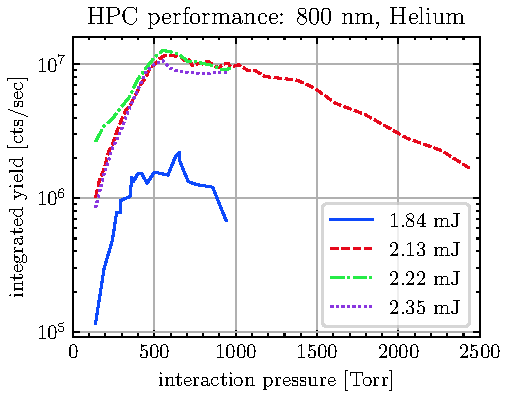
\includegraphics[width=0.75\textwidth]{figures/chap3/HPC_P_scaling_He800.pdf}
	\caption{Total harmonic yield as function of interaction pressure in the HPC.}
	\label{fig:HPC_performance}
\end{figure}

\begin{figure}
	\centering
	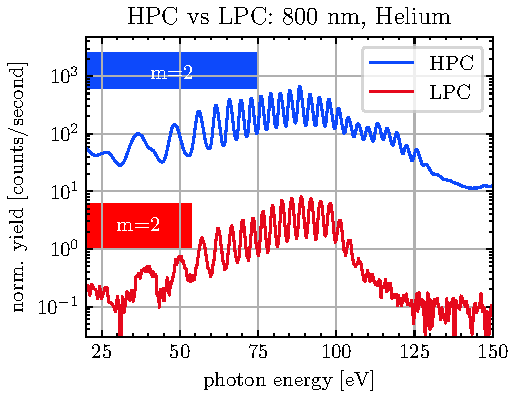
\includegraphics[width=0.75\textwidth]{figures/chap3/HPC_vs_LPC_800He.pdf}
	\caption{Comparison of the LPC and the HPC in helium at 800 nm. Generation conditions for each were optimized (LPC: 17 Torr interaction pressure, 1.85 mJ; HPC: 650 Torr, 2.13 mJ) in helium at 800 nm. The HPC extends the cutoff from 104 eV to 132 eV and increases the XUV brightness by roughly 100x across the spectrum. Note that harmonics with energies less than half the cutoff are contaminated by \nth{2} order diffraction from the XUV spectrometer's grating.}
	\label{fig:HHG-HPCvsLPCHPC}
	% plot made in \Python Scripts\HPC\HPCvLPC_comparison.py
\end{figure}

The pressure scaling of the HPC is shown in \cref{fig:HPC_performance}. Unlike the LPC, we can see a maximum in the harmonic yield with respect to pressure. Although the y-axis scale for \cref{fig:LPC_performance,fig:HPC_performance} is arbitrary, they are in the same units and therefore are comparable. We can see that the total harmonic yield of the HPC exceeds that of the LPC by about 2 orders of magnitude.

HHG yields at higher pressures are lower than otherwise expected, most likely due to increased XUV absorption in the PM region, and perhaps non-ideal IR propagation before the focus. ie, the increased pressure messes up the pulse, or the XUV is reabsorbed after it is made.

A comparison between the LPC and the HPC is shown in \cref{fig:HHG-HPCvsLPCHPC}.

The performance increase of the HPC comes from an increased pressure-length product, which is primarily due to the inner pipe's geometry and the differential pumping afforded by the outer shroud. We have tested the HPC with backing pressures up to 150 psig, which was previously only possible in our lab using expensive and unreliable pulsed valves.


- limited pump speed $\rightarrow$ differential pumping is required


harmonic yield results

advantages: much brighter due to pressure-length product. future application: can operate in low-pressure mode and reduce downstream generation gas contamination of target chamber.

disadvantages: difficult to align and initially install (once it's installed, alignment is easy). messed up mode. HHG instability at higher pressures.

pictures of the HPC.



\subsection{Pulsed Amsterdam Piezovalve}
% piezovalve yield vs pressure: C:\testdata\2019_10_10

\begin{figure}
	\centering
	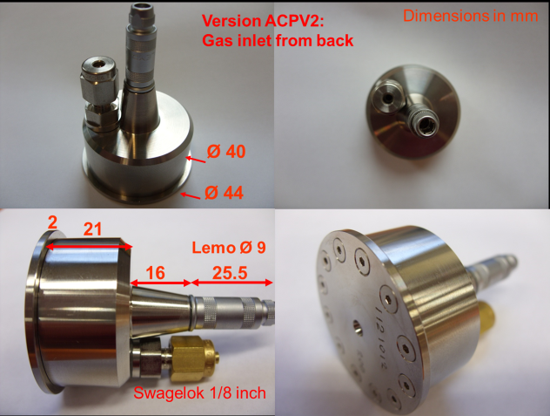
\includegraphics[width=0.75\textwidth]{figures/chap3/piezovalve_picture.png}
	\caption{Amsterdam Piezo Valve. Gas exits from the center of the front face (flat side).}
	\label{fig:piezovalve_picture}
	% picture supplied by andrew piper
\end{figure}

\begin{figure}
	\centering
	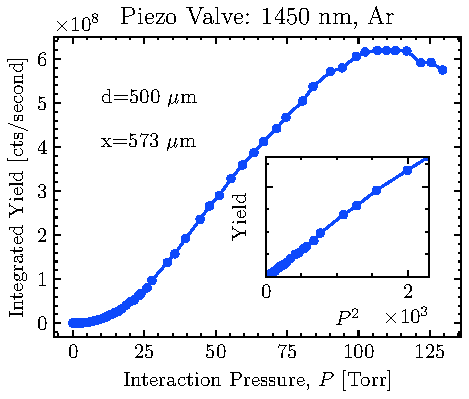
\includegraphics[width=0.75\textwidth]{figures/chap3/piezovalve_pscan.pdf}
	\caption{integrated harmonic yield vs pressure. inset: yield vs square of pressure, showing excellent quadratic behavior. argon, 1450 nm.}
	\label{fig:piezovalve_pscan}
	% plot made in \Python Scripts\HPC\piezovalve_1450nm.py
\end{figure}

\begin{figure}
	\centering
	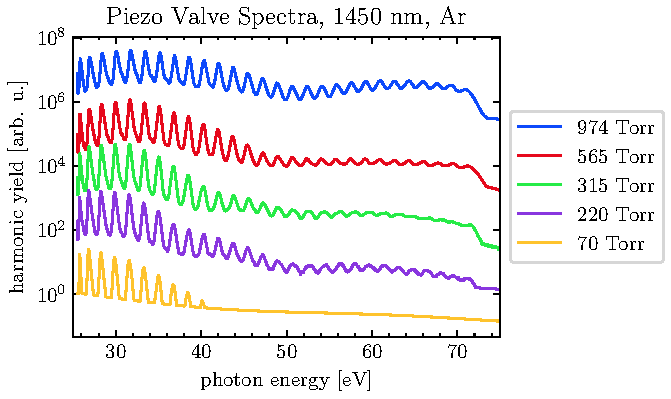
\includegraphics[width=0.9\textwidth]{figures/chap3/piezovalve_spectra.pdf}
	\caption{piezovalve spectra vs pressure. argon, 1450 nm.}
	\label{fig:piezovalve_spectra}
	% plot made in \Python Scripts\HPC\piezovalve_1450nm.py
\end{figure}

commercial pulsed valve. 

500 micron diameter nozzle

Amsterdam Piezo Valve. 


settings and equipment we used for this experiment: $75 \ \mu \textrm{s}$ opening time, 150 V. guestimate x = 250 micron on-axis distance from aperture to laser focus

delay introduced by Quantum Composer.

thanks to andrew piper for letting us use his piezovalve.

the piezo valve is shown in \cref{fig:piezovalve_picture}.

pressure scaling of total harmonic yield is shown in \cref{fig:piezovalve_pscan}.

evolution of spectra / shape of spectra changes with pressure, as shown in \cref{fig:piezovalve_spectra}. this is due to the photon energy dependence of phase matching conditions. this is typical for all gas sources.

for more detail and characterization of the piezo valve, see andrew piper's dissertation \cite{piperAndrewPiperDissertation2022}.



\section{Characterization of XUV Source}

\subsection{Knife Edge Measurements}

\begin{figure}
	\centering
	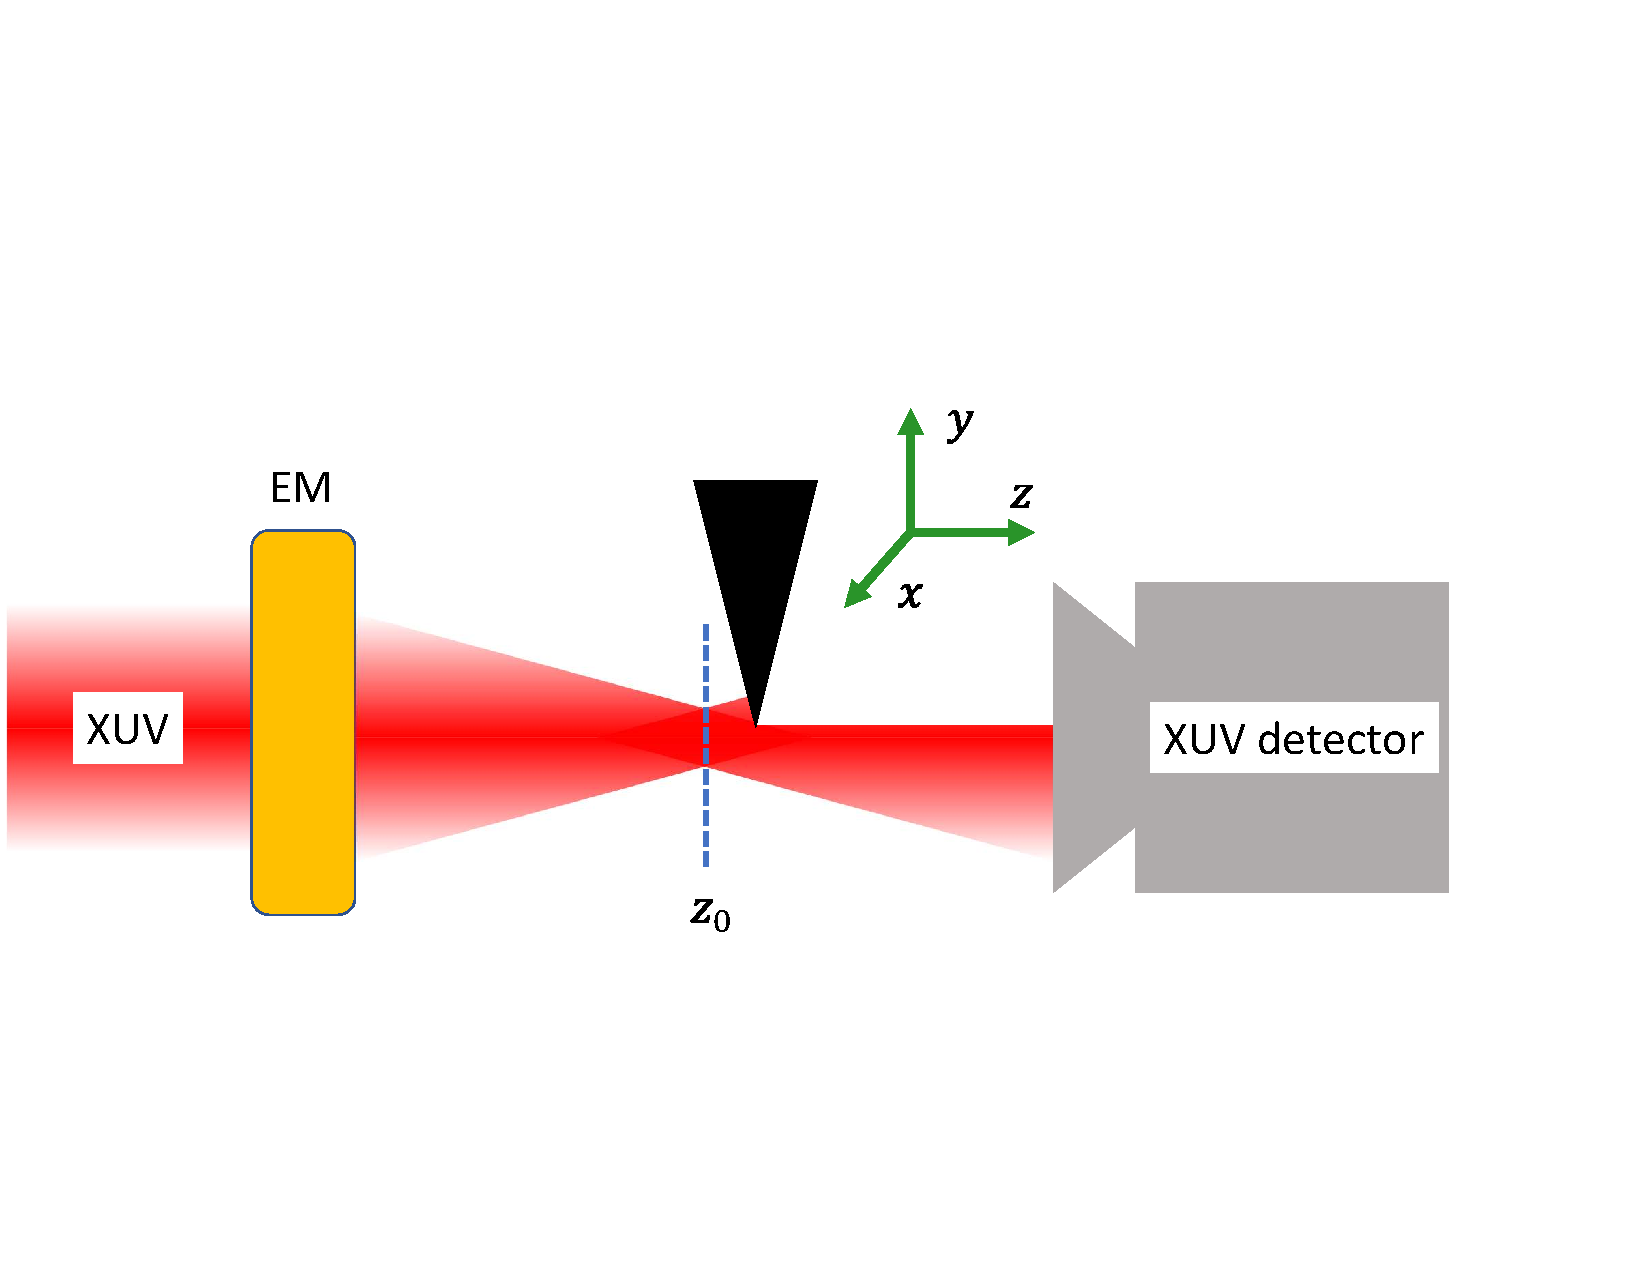
\includegraphics[width=0.75\textwidth]{figures/chap3/knife_edge_cartoon.pdf}
	\caption{Schematic of XUV knife edge measurement. EM: ellipsoidal mirror, $z_0$: XUV focal plane.}
	\label{fig:knife_edge_cartoon}
\end{figure}

\begin{figure}
	\centering
	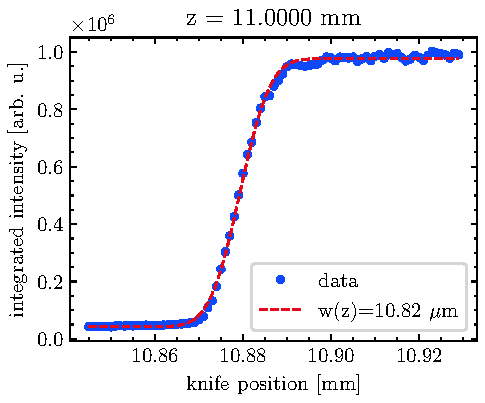
\includegraphics[width=0.75\textwidth]{figures/chap3/XUV_focus_knife_edge.pdf}
	\caption{A typical XUV knife edge measurement near the focal plane. The sample motor position is $k=11.0000$ mm. A fit to equation \cref{eqn:knife_edge} yields a beam waist of 10.82 $\mu$m at this position.}
	\label{fig:XUV_focus_knife_edge}
	% dataset: C:\testdata\2019_08_23\knife\11.0000
	% python file: \Python Scripts\Spectrometer\test\knife_edge.py
\end{figure}

\begin{figure}
	\centering
	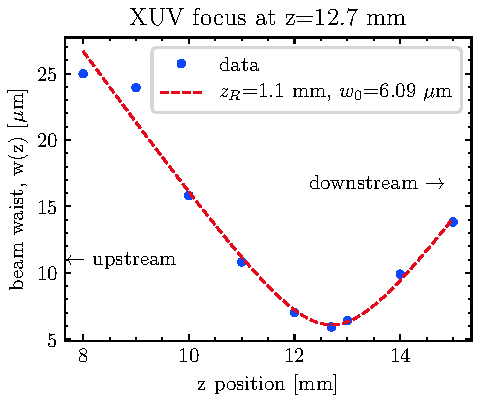
\includegraphics[width=0.75\textwidth]{figures/chap3/XUV_waist_vs_k.pdf}
	\caption{Evolution of XUV beam waist as a function of propagation direction, $z$. The Rayleigh range $z_R$ and beam waist $w_0$ are extracted from the fit to \cref{eqn:beam_waist_evolution}.}
	\label{fig:XUV_waist_vs_k}
	% question: what is $M^2$ value of the XUV?. or, does w0 and zR change with XUV wavelength?
	% dataset: C:\testdata\2019_08_23\knife\11.0000
	% python file: \Python Scripts\Spectrometer\test\knife_edge.py
\end{figure}

We characterize the XUV focus in the target chamber by performing knife edge measurements at different $k$-positions, as depicted in \cref{fig:knife_edge_cartoon}. We use the interior angled edge of the Si frame on a broken sample heterostructure as a knife edge (see \cref{fig:Sample_Geometry}). This frame makes an excellent knife edge as it has a very well-defined geometry and fits in the sample holder. Recalling Gaussian optics, the assumed profile of the XUV beam is:
\begin{equation}
I(x,y,z) = I_0 \left( \frac{w_0}{w(z)} \right)^2 \exp \left( -2 \frac{ (x-x_0)^2 + (y-y_0)^2 }{w(z)^2} \right),
\end{equation}
using the coordinate system defined in \cref{fig:knife_edge_cartoon}. The XUV focus is at position $(x_0,y_0,z_0)$. The beam waist $w(z)$ will evolve as:
\begin{equation}
w(z) = w_0 \sqrt{ 1 + \left( \frac{z-z_0}{z_R} \right)^2 },
\label{eqn:beam_waist_evolution}
\end{equation}
where $z_R$ is the Rayleigh range. If we use the knife edge to block the transmission as depicted in \cref{fig:knife_edge_cartoon}, then the transmitted power will be:
\begin{equation}
P(x, z) = P_0 + \frac{P_{max}}{2} \left( 1 - \erf \left( \frac{\sqrt{2}(x-x_0)}{w(z)} \right) \right),
\label{eqn:knife_edge}
\end{equation}
where $x$ is the insertion of the knife in the beam, $z$ represents the location of the knife plane in the propagation direction, and $\erf$ is the error function.

A typical knife edge measurement is shown \cref{fig:XUV_focus_knife_edge}. In this measurement, the knife edge is translated across the XUV spot in 1 $\mu$m steps until the XUV light is completely blocked. A 2D spectrum is saved at each knife edge position. Each image is background subtracted, normalized and summed (integrating over all divergences and wavelengths), which yields the XUV flux as a function of knife position. The resulting curve is fit to \cref{eqn:knife_edge} and the beam waist $w(z)$ is extracted for this $z$-position.

The knife edge measurement is repeated at different $z$-positions until enough data has been acquired to determine the focal plane. The evolution of the XUV beam waist is shown in \cref{fig:XUV_waist_vs_k}. In this figure, the beam waist has been fit to \cref{eqn:beam_waist_evolution} to determine the focal plane $z_0$, the Rayleigh range $z_R$ and the beam waist $w_0$. In both figures, a reasonably good fit is obtained, indicating that the XUV light has a Gaussian spatial profile near the focus.


\subsection{harmonic yield stability}

\subsection{XUV spectra optimized for various HHG conditions}

\subsection{Measured Transmission of Metallic Filters}

\subsection{Ground State Measurements of Condensed Matter Samples}

\section{characterization of interferometric stability}

\section{MCP response}
% MCP voltage data taken on 2019_10_07.
scaling of yield and noise with respect to MCP voltage
